\documentclass[11pt,a4paper]{article}

\usepackage[utf8]{inputenc}
\usepackage{lmodern}
\usepackage[T1]{fontenc}
\IfFileExists{french.ldf}{\usepackage[french]{babel}}{}
\renewcommand{\contentsname}{Table des matières}
\renewcommand{\figurename}{Figure}
\renewcommand{\tablename}{Tableau}
\renewcommand{\refname}{Références}
\usepackage{geometry}
\usepackage{graphicx}
\usepackage{xcolor}
\usepackage{amsmath,amssymb}
\usepackage{booktabs}
\usepackage{tabularx}
\usepackage{array}
\usepackage{float}
\usepackage{caption}
\usepackage{enumitem}
\usepackage{fancyhdr}
\usepackage{listings}
\usepackage{titlesec}
\usepackage{indentfirst}
\usepackage{hyperref}

\geometry{margin=2.4cm,headheight=15pt}
\definecolor{titreNoir}{HTML}{000000}
\definecolor{fondCommandes}{HTML}{FAF5EF}
\definecolor{bordCommandes}{HTML}{79523A}
\hypersetup{
  colorlinks=true,
  linkcolor=titreNoir,
  urlcolor=titreNoir,
  citecolor=titreNoir,
  pdftitle={Compte-rendu - Projet Analyse de la structure des membranes lipidiques},
  pdfauthor={BERNARD Valentin, BRAHAM Amyne, FOURNAISE Antoine, ZAMOUM Tassadit},
}
\setlength{\parindent}{1.4em}
\setlength{\parskip}{0pt}
\linespread{1.08}
\raggedbottom
\setlist[itemize]{leftmargin=*,topsep=2pt,itemsep=2pt}
\setlist[enumerate]{leftmargin=*,topsep=2pt,itemsep=2pt}
\renewcommand{\arraystretch}{1.25}
\titleformat{\section}{\Large\bfseries}{\thesection\ --}{0.5em}{}
\titleformat{\subsection}{\large\bfseries}{\thesubsection\ --}{0.5em}{}
\titleformat{\subsubsection}{\normalsize\bfseries}{\thesubsubsection\ --}{0.5em}{}
\titleformat{\paragraph}[block]{\normalsize\bfseries}{}{0pt}{}
\titlespacing*{\section}{0pt}{1.6em}{0.9em}
\titlespacing*{\subsection}{0pt}{1.3em}{0.6em}
\titlespacing*{\paragraph}{0pt}{1.1em}{0.4em}
\captionsetup{font=small,labelfont=bf,justification=centering,width=0.9\textwidth,skip=6pt}
\captionsetup[table]{font=small,labelfont=bf,justification=raggedright,singlelinecheck=false,width=\textwidth,skip=5pt,position=top}
\captionsetup[lstlisting]{font=small,labelfont=bf,justification=centering,skip=6pt}
\lstdefinestyle{terminal}{
  basicstyle=\ttfamily\small,
  backgroundcolor=\color{fondCommandes},
  frame=single,
  rulecolor=\color{bordCommandes},
  breaklines=true,
  columns=fullflexible,
  keepspaces=true,
  showstringspaces=false,
  xleftmargin=0.3em,
  xrightmargin=0.3em,
  extendedchars=true,
  aboveskip=1.1em,
  belowskip=1.1em,
  literate={é}{{\'e}}1 {è}{{\`e}}1 {ê}{{\^e}}1 {à}{{\`a}}1 {ç}{{\c{c}}}1
           {É}{{\'E}}1 {ô}{{\^o}}1 {î}{{\^i}}1 {ù}{{\`u}}1 {œ}{{\oe}}1 {û}{{\^u}}1 {µ}{{$\mu$}}1
}
\lstset{style=terminal}
\makeatletter\newcommand{\tabinput}[1]{\@@input #1 }\makeatother

% membres du groupe, par ordre alphabetique du nom de famille
\newcommand{\auteurUn}{\textsc{Bernard} Valentin}
\newcommand{\auteurDeux}{\textsc{Braham} Amyne}
\newcommand{\auteurTrois}{\textsc{Fournaise} Antoine}
\newcommand{\auteurQuatre}{\textsc{Zamoum} Tassadit}
\newcommand{\enseignant}{\textsc{Crowet} Jean-Marc}
\newcommand{\formation}{Master 2 Calcul Haute Performance et Simulation (CHPS)}
\newcommand{\anneeUniv}{2026--2027}
\newcommand{\dateRapport}{25 novembre 2026}

\pagestyle{fancy}
\fancyhf{}
\fancyhead[L]{\small Éléments de bioinformatique : le HPC en biologie}
\fancyhead[R]{\small Compte-rendu -- Projet membranes lipidiques}
\fancyfoot[C]{\thepage}
\renewcommand{\headrulewidth}{0pt}
\renewcommand{\footrulewidth}{0pt}

\newcommand{\TPTrames}{1001}
\newcommand{\TPLipides}{3040}
\newcommand{\TPAtomes}{83\,095}
\newcommand{\TPLecture}{2,35}
\newcommand{\TPDetect}{29,5}
\newcommand{\TPVq}{1,31}
\newcommand{\TPVtot}{1,31}
\newcommand{\TPSeq}{1,260}
\newcommand{\TPPar}{0,278}
\newcommand{\TPSeqHz}{793}
\newcommand{\TPParHz}{3599}
\newcommand{\TPExtSeq}{126}
\newcommand{\TPExtPar}{28}
\newcommand{\TPFat}{28,7}
\newcommand{\TPLF}{87,3}
\newcommand{\TPAccFat}{99,75}
\newcommand{\TPAccFatMin}{99,18}
\newcommand{\TPChgMoy}{5}
\newcommand{\TPAccRef}{n/a}
\newcommand{\TPFusions}{0}
\newcommand{\TLTrames}{21}
\newcommand{\TLLipides}{3040}
\newcommand{\TLAtomes}{83\,095}
\newcommand{\TLLecture}{2,34}
\newcommand{\TLDetect}{28,9}
\newcommand{\TLVq}{1,26}
\newcommand{\TLVtot}{0,03}
\newcommand{\TLSeq}{1,267}
\newcommand{\TLPar}{0,273}
\newcommand{\TLSeqHz}{789}
\newcommand{\TLParHz}{3666}
\newcommand{\TLExtSeq}{127}
\newcommand{\TLExtPar}{27}
\newcommand{\TLFat}{0,6}
\newcommand{\TLLF}{1,8}
\newcommand{\TLAccFat}{99,75}
\newcommand{\TLAccFatMin}{99,61}
\newcommand{\TLChgMoy}{307}
\newcommand{\TLAccRef}{n/a}
\newcommand{\TLFusions}{0}
\newcommand{\TDTrames}{11}
\newcommand{\TDLipides}{3072}
\newcommand{\TDAtomes}{36\,864}
\newcommand{\TDLecture}{1,09}
\newcommand{\TDDetect}{25,1}
\newcommand{\TDVq}{1,27}
\newcommand{\TDVtot}{0,01}
\newcommand{\TDSeq}{1,278}
\newcommand{\TDPar}{0,259}
\newcommand{\TDSeqHz}{783}
\newcommand{\TDParHz}{3865}
\newcommand{\TDExtSeq}{128}
\newcommand{\TDExtPar}{26}
\newcommand{\TDFat}{0,4}
\newcommand{\TDLF}{0,9}
\newcommand{\TDAccFat}{99,97}
\newcommand{\TDAccFatMin}{99,93}
\newcommand{\TDChgMoy}{1}
\newcommand{\TDAccRef}{100,00}
\newcommand{\TDFusions}{0}
\newcommand{\TNcpu}{12}


\begin{document}
\hypersetup{pageanchor=false}

% -------------------- Page de garde --------------------
\begin{titlepage}
\thispagestyle{empty}
\centering
\vspace*{0.65cm}

\includegraphics[width=0.46\textwidth,keepaspectratio]{figures/logo-urca-officiel.png}\\[1.05cm]
{\Large Université de Reims Champagne-Ardenne\par}
\vspace{0.35cm}
{\large \formation\par}
\vspace{0.35cm}
{\normalsize UE Éléments de bioinformatique : utilisation du HPC dans la biologie (CHPS1001)\par}
\vspace{1.45cm}
{\Huge\bfseries\color{titreNoir} Compte-rendu\par}
\vspace{0.35cm}
{\LARGE Projet : analyse de la structure\\[0.15cm]
des membranes lipidiques\par}
\vspace{0.3cm}
{\large Assignation des lipides à leur feuillet\par}
\vspace{1.5cm}
{\normalsize\bfseries Membres du groupe\par}
\vspace{0.3cm}
{\large
\auteurUn\par\vspace{0.12cm}
\auteurDeux\par\vspace{0.12cm}
\auteurTrois\par\vspace{0.12cm}
\auteurQuatre\par}
\vspace{0.9cm}
{\normalsize\bfseries Enseignant\par}
\vspace{0.3cm}
{\large \enseignant\par}
\vfill
{\large Année universitaire \anneeUniv\par}
{\normalsize \dateRapport\par}
\end{titlepage}

\hypersetup{pageanchor=true}
\sloppy
\setcounter{page}{1}
\begingroup
\setcounter{tocdepth}{2}
\tableofcontents
\endgroup
\clearpage

% ======================================================================
\section*{Introduction}
\addcontentsline{toc}{section}{Introduction}
Avant toute analyse d'une membrane simulée par dynamique moléculaire (aire par lipide, épaisseur, interactions
lipide/protéine\ldots), il faut savoir à quel feuillet appartient chaque lipide, et le refaire à chaque trame
puisque des lipides peuvent passer d'un feuillet à l'autre. Pour une bicouche plane, la coordonnée selon la normale
suffit~; pour une vésicule ou une membrane ondulée, il faut une méthode géométrique plus générale. L'énoncé demande~:
\begin{enumerate}
\item une première version utilisant les graphes avec une recherche de seuil automatisée~;
\item une version ne nécessitant pas la définition d'un atome de référence par lipide au préalable~;
\item une version prenant en compte l'orientation des lipides et la normale locale à chaque lipide~;
\item une version finale fondée sur les éléments nécessaires et suffisants, en justifiant les choix
(fiabilité, temps de calcul, robustesse)~;
\item l'application de la version finale à une trajectoire complète, avec mesure du temps de calcul~;
\item la comparaison des versions avec LeafletFinder (MDAnalysis) et FATSLiM, sur les structures et sur la
trajectoire.
\end{enumerate}

Nous avons développé en C++ (OpenMP) un outil qui réalise ces quatre versions. Sur les sept structures fournies, la
version finale retrouve la référence à 99,77--100\,\%~: toutes les erreurs résiduelles sont des molécules de
cholestérol ou de diacylglycérol situées au plan médian de la bicouche, en cours de \emph{flip-flop}. Elle analyse
une structure en 0,03 à 7,5\,ms sur un seul cœur, soit 28 à 250 fois plus vite que FATSLiM et 59 à 185 fois plus
vite que LeafletFinder, qui échoue par ailleurs sur les membranes plasmiques avec son seuil par défaut. Appliquée à la
trajectoire fournie (bicouche PIPC/GCER/cholestérol en présence de surfactine, 3040 lipides, \TPTrames~trames), elle
analyse une trame en \TPVq\,ms, soit \TPSeqHz~trames/s sur un cœur et \TPParHz~trames/s sur \TNcpu~threads, en
accord à \TPAccFat\,\% avec FATSLiM.

Les sections~\ref{sec:v1} à~\ref{sec:v4} décrivent les versions 1 à 4, la section~\ref{sec:struct} les compare sur
les structures (point~6) et la section~\ref{sec:traj} traite la trajectoire (points~5 et~6).

%=====================================================================
\section{Matériel et environnement}
%=====================================================================
\subsection{Données}
Les sept structures fournies (format GRO, archive \texttt{Projet3.zip}) et le nombre de lipides de référence
(fichiers \texttt{leaflets.txt}) sont résumés au tableau~\ref{tab:sys}. Elles couvrent des représentations
\emph{united-atom} (UA) et gros grains (CG, Martini), des bicouches planes avec peptides, des vésicules et deux
membranes plasmiques de 63 à 65 types de lipides (cholestérol, sphingolipides, glycolipides, phosphoinositides,
diacylglycérols, céramides\ldots). Les boîtes sont orthorhombiques sauf \texttt{dppc\_vesicle} (boîte triclinique,
dodécaèdre rhombique).

\begin{table}[H]\centering\small
\caption{Systèmes étudiés. « Lipides » = molécules reconnues comme lipides par notre programme~; « Réf. » = lipides
présents dans le fichier de référence. Les 42 lipides de \texttt{dppc\_vesicle} absents de la référence sont des
lipides libres (petits agrégats dans le solvant).}\label{tab:sys}
\begin{tabular}{|l|r|r|r|}\hline
\textbf{Système} & \textbf{Atomes} & \textbf{Lipides} & \textbf{Réf.}\\\hline
\tabinput{tables/systemes.tex}
\end{tabular}
\end{table}

\textbf{Trajectoire.} La trajectoire fournie pour le cas d'application final (dossier \texttt{Surfactine-R1/})
est une simulation GROMACS en champ de forces Martini~3 d'une bicouche plane construite avec INSANE, de même
composition dans les deux feuillets (PIPC/GCER/CHOL 60:20:20, soit 1824 PIPC, 608 glucosylcéramides GCER et 608
cholestérols~: 3040 lipides), en présence de 96 molécules de \textbf{surfactine} (lipopeptide bactérien~: une queue
\texttt{S14} et sept acides aminés), placées initialement de part et d'autre de la membrane, dans 43\,349 billes
d'eau et 2754 ions (83\,095 particules, boîte de $29{,}7\times29{,}7\times9{,}7$\,nm). Le dossier contient les étapes
de préparation (minimisation, équilibration), une phase où les surfactines sont tirées vers la membrane
(\texttt{prod1}, 5\,ns) et la production (\texttt{prod}, 20\,µs, pas de 20\,fs). Les trajectoires utilisables sont
résumées au tableau~\ref{tab:trajdata}~; \texttt{prod\_pep.xtc} ne contient que les peptides (pas de lipides) et
\texttt{prod.trr} est tronqué (61 trames lisibles sur environ 400, fichier incomplet).

\begin{table}[H]\centering\small
\caption{Trajectoires analysées («~Surf.~»~: trajectoires du dossier \texttt{Surfactine-R1}). La vésicule DPPC (11 trames, données de test de FATSLiM) a servi à mettre au point
la chaîne de traitement avant de disposer de la trajectoire du cours.}\label{tab:trajdata}
\begin{tabular}{|l|r|r|r|r|}\hline
\textbf{Trajectoire} & \textbf{Trames} & \textbf{Durée} & \textbf{Lipides} & \textbf{Particules}\\\hline
\tabinput{tables/traj_donnees.tex}
\end{tabular}
\end{table}

\subsection{Machine et logiciels}
Portable Intel Core i7-1255U (2 cœurs performance + 8 cœurs efficacité, 12 threads), 15\,Go de RAM, Fedora~43.
Déjà présents~: GCC~15.3 (OpenMP), Python~3.14, NumPy, VMD, \LaTeX. Installés pour le projet (sans droits
administrateur, dans le dossier du projet)~:
\begin{itemize}
\item \texttt{.venv/}~: environnement Python~3.14 avec MDAnalysis~2.11 (LeafletFinder), SciPy, NetworkX,
Matplotlib~;
\item \texttt{.venv-fatslim/}~: FATSLiM~0.2.2 compilé dans un environnement Python~3.9 dédié (installé avec
\texttt{uv}), FATSLiM n'étant pas compatible avec Python~3.14 ni NumPy~2.
\end{itemize}

\subsection{Mesure de la fiabilité}
Pour chaque méthode, les feuillets trouvés sont associés aux feuillets de référence de manière gloutonne (le plus
grand groupe trouvé prend le feuillet de référence avec lequel il partage le plus de lipides, etc.). L'\emph{accord}
est la fraction des lipides de référence placés dans le bon feuillet~; un lipide non assigné, ou placé dans un
groupe surnuméraire, compte comme une erreur. Nous constatons que FATSLiM retrouve exactement la référence sur six
des sept structures~: les fichiers \texttt{leaflets.txt} ont très vraisemblablement été produits avec FATSLiM, ce
qui avantage mécaniquement cet outil dans la comparaison.

\subsection{Mesure du temps}
Les temps rapportés pour nos versions sont des temps d'analyse d'une trame (coordonnées déjà en mémoire, lecture du
fichier exclue), minimum de plusieurs répétitions, sur un seul thread sauf mention contraire. Pour LeafletFinder,
il s'agit du temps de l'appel Python (recherche de voisins + composantes connexes)~; pour FATSLiM, du temps par trame
affiché par le logiciel (résolution 1\,ms). Les étapes faites une seule fois par système (lecture de la topologie,
détection des atomes de référence en V2--V4) sont données à part.

Les mesures finales ont été faites sur un ordinateur portable fonctionnant sur batterie (gouverneur
\texttt{powersave}), avec d'autres applications ouvertes~: les temps absolus sont donc pessimistes et un peu
dispersés (de l'ordre de 10--20\,\% d'une exécution à l'autre). Toutes les méthodes ayant été mesurées dans les
mêmes conditions, les comparaisons restent valables. Le script \texttt{resultats/relance\_tout.sh} refait
l'ensemble des mesures.

%=====================================================================
\section{Socle commun à toutes les versions}
%=====================================================================
Toutes les versions partagent un même code C++ (\texttt{src/leaflet.cpp}, environ 1300 lignes), compilé en
exécutable (\texttt{bin/leaflet}) et en bibliothèque partagée (\texttt{lib/libleaflet.so}, appelée depuis Python
par \texttt{ctypes} pour les comparaisons).

\paragraph{Topologie.} Une molécule est une suite d'atomes consécutifs de même numéro et même nom de résidu (ce
qui gère le repliement des numéros au-delà de 99\,999 dans les fichiers GRO). Le solvant, les ions et les acides
aminés sont exclus par une courte liste de noms~; toutes les autres molécules sont des lipides. Les lipides sont
regroupés en \emph{types} (nom + nombre d'atomes), ce qui permet de faire une seule fois par type les opérations
coûteuses.

Cette définition par résidu est valable pour les sept structures, mais pas pour la trajectoire~: en Martini~3, un
glucosylcéramide est écrit sur deux résidus (sucre et céramide) et une surfactine sur huit. Le programme accepte donc
aussi le découpage exact en molécules donné par le fichier de topologie GROMACS (\texttt{.tpr}, lu avec MDAnalysis~;
option \texttt{--molsizes} de l'exécutable), et une liste de résidus à exclure (option \texttt{-x}). La surfactine,
lipopeptide et non lipide membranaire, est exclue de l'assignation~; les mêmes lipides et les mêmes atomes de tête
sont donnés à LeafletFinder et à FATSLiM.

\paragraph{Conditions périodiques (PBC).} Les positions sont manipulées en coordonnées fractionnaires
$\mathbf f=\mathbf r\,\mathbf H^{-1}$, ce qui traite de façon unique les boîtes orthorhombiques et tricliniques.
Chaque molécule est reconstituée entière autour de son atome de tête par image minimale.

\paragraph{Recherche de voisins.} Une grille de cellules (côté $\geq$ seuil $r_c$) en coordonnées fractionnaires,
avec tri des points par cellule (tri par comptage, $O(N)$) et parcours du demi-voisinage (13 cellules + la cellule
elle-même), donne toutes les paires à distance $<r_c$ en $O(N)$. Les images périodiques sont explicites, ce qui reste
correct pour les petites boîtes (moins de trois cellules par direction). La boucle sur les cellules est parallélisée
avec OpenMP. Chaque paire conserve son vecteur de séparation, réutilisé ensuite pour les normales.

\paragraph{Composantes connexes.} Le graphe n'est jamais construit explicitement~: chaque arête retenue est
insérée dans une structure Union-Find (compression de chemin, union par taille), en temps quasi linéaire. Les
composantes de plus de $\max(10,\,0{,}02N)$ lipides sont les feuillets (triés par taille décroissante)~; les
lipides des petites composantes sont des \emph{orphelins}, rattachés ensuite au feuillet de leur plus proche voisin
assigné.

\paragraph{Optimisations.} Lecture GRO maison (fichier lu en un bloc, conversion des nombres à largeur fixe, largeur
des champs détectée automatiquement), tampons réutilisés d'une trame à l'autre, et réglage de l'allocateur
(\texttt{mallopt}) pour éviter que les tableaux de quelques Mo soient rendus au système puis remis à zéro par le
noyau à chaque trame~: le profilage (\texttt{perf}) montrait que cela coûtait environ 30\,\% du temps d'analyse.

%=====================================================================
\section{Version 1~: graphe et recherche automatique du seuil}\label{sec:v1}
%=====================================================================
\paragraph{Principe.} Chaque lipide est représenté par un atome de référence (le phosphate~: \texttt{PO4} en CG,
\texttt{P}/\texttt{P8} en UA~; \texttt{ROH} pour le cholestérol, \texttt{AM1} pour les céramides et glycolipides,
\texttt{GL1} pour les diacylglycérols, \texttt{CP} pour les phosphoinositides). Deux lipides sont reliés si leurs
atomes de référence sont à moins d'un seuil $c$~; les feuillets sont les composantes connexes.

\paragraph{Seuil automatique.} Le comportement du graphe en fonction de $c$ est illustré
figure~\ref{fig:seuil}~: pour $c$ trop petit, le graphe est fragmenté~; il existe ensuite un \emph{plateau} où les
deux feuillets sont formés mais séparés~; pour $c$ trop grand, des arêtes traversent la bicouche et tout fusionne.
La V1 détecte ce plateau en un seul passage~:
\begin{enumerate}
\item recherche de toutes les paires à moins de $r_{\max}=2{,}5$\,nm (une seule recherche de voisins)~;
\item classement des paires par tranches de distance de 0,02\,nm (tri par comptage)~;
\item insertion des arêtes par distance croissante dans l'Union-Find (équivalent à un regroupement hiérarchique
à lien simple), en suivant la taille des deux plus grandes composantes après chaque tranche~;
\item une fusion est \emph{significative} si la plus petite des deux composantes fusionnées dépasse 10\,\% des
lipides~: la dernière fusion significative est celle des deux feuillets et marque la fin du plateau~;
le début du plateau est la première tranche où les deux plus grandes composantes atteignent 90\,\% de leur taille
finale~;
\item le seuil retenu est le milieu du plateau (marge maximale des deux côtés).
\end{enumerate}
Si aucune fusion des feuillets n'a lieu avant $r_{\max}$ (cas des vésicules, dont les feuillets sont plus écartés),
la fin du plateau est $r_{\max}$.

\begin{figure}[H]\centering
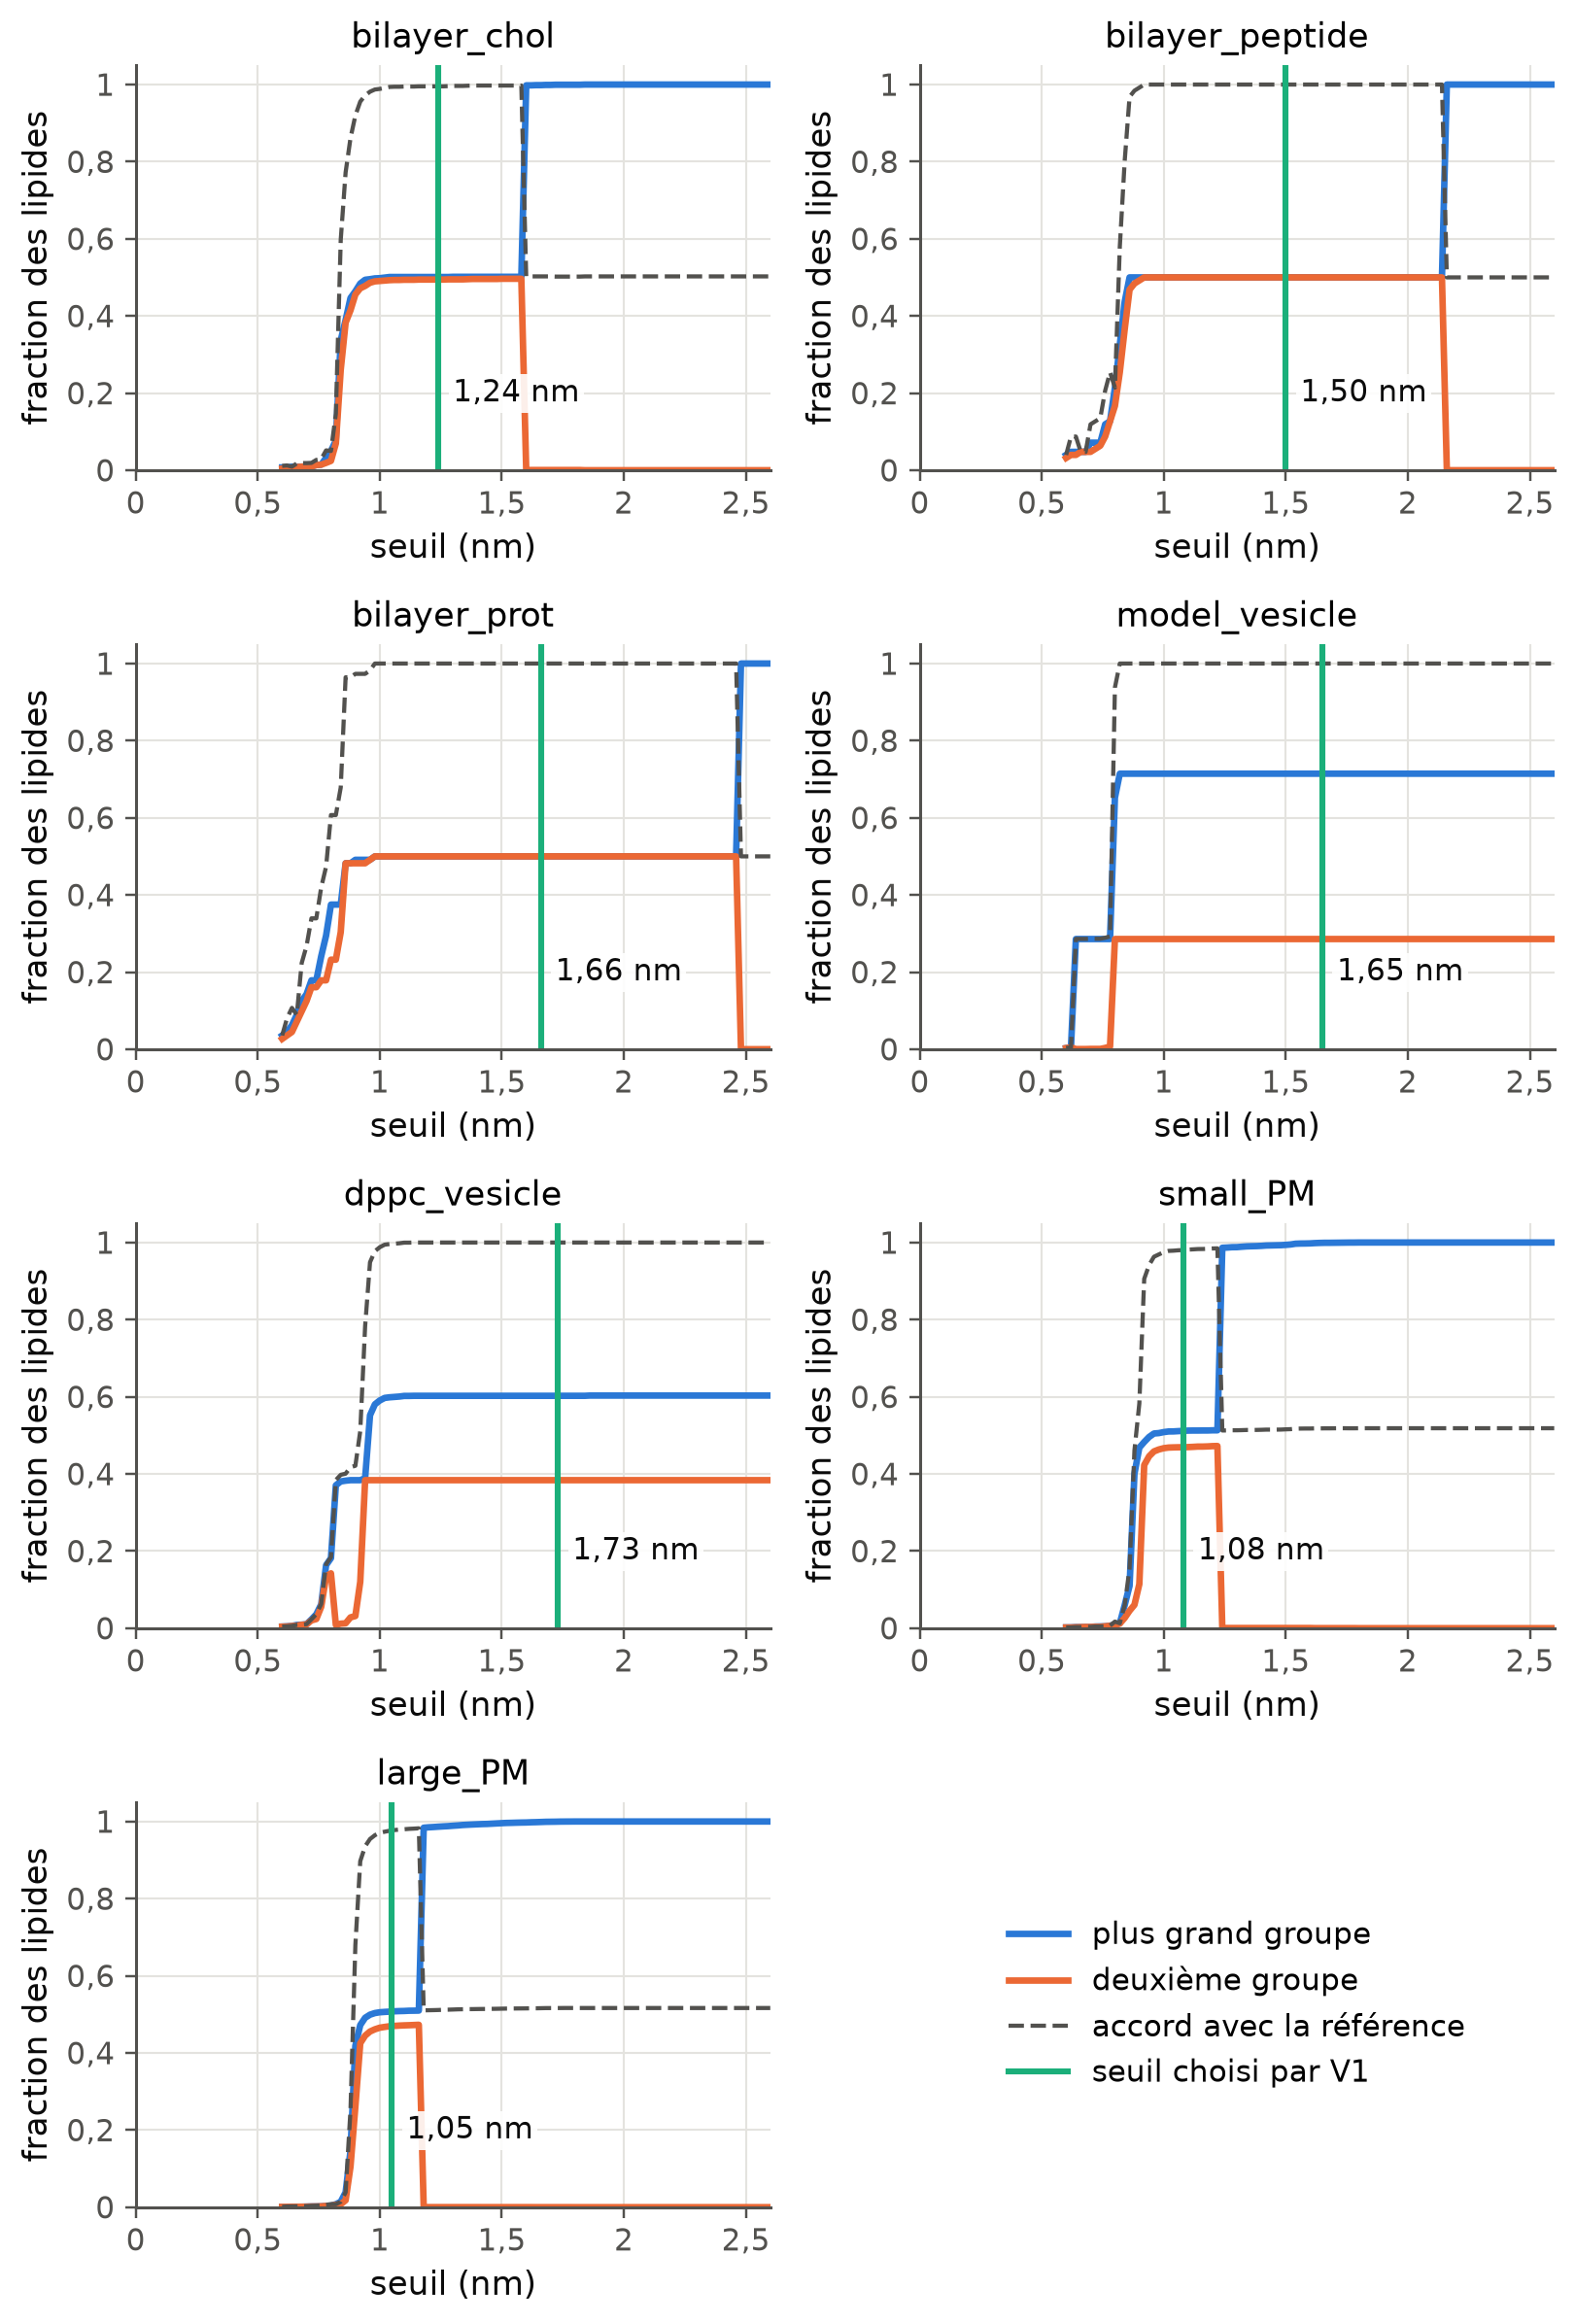
\includegraphics[width=0.82\textwidth]{../../resultats/figures/fig_balayage_seuil.png}
\caption{Taille (fraction des lipides) des deux plus grandes composantes connexes du graphe des atomes de
référence en fonction du seuil, et accord avec la référence (tirets). La ligne verte est le seuil choisi
automatiquement par la V1. Le plateau où les deux feuillets sont séparés est large pour les bicouches simples et
les vésicules, mais très étroit pour les membranes plasmiques (environ 0,95--1,2\,nm).}\label{fig:seuil}
\end{figure}

\paragraph{Résultats.} Les seuils trouvés (tableau~\ref{tab:seuils}) tombent toujours dans le plateau~: la V1
atteint 99,72 à 100\,\% d'accord sur les sept structures (tableau~\ref{tab:accord}). La figure~\ref{fig:seuil}
montre aussi la \textbf{limite} de l'approche~: sur les membranes plasmiques, le plateau ne fait que
$\approx$\,0,25\,nm, car les petites têtes enfouies (cholestérol, diacylglycérols) et le cholestérol en cours de
\emph{flip-flop} forment des ponts entre feuillets~; un seuil fixe (par exemple 1,5\,nm, valeur par défaut de
LeafletFinder) y échoue complètement. La recherche automatique est donc indispensable dans cette approche, et le
résultat dépend du choix, fait à la main, de l'atome de référence de chaque type de lipide.

%=====================================================================
\section{Version 2~: sans atome de référence défini au préalable}\label{sec:v2}
%=====================================================================
\paragraph{Principe.} La V2 détermine elle-même, pour chaque \emph{type} de lipide, l'atome qui joue le rôle de
groupe de tête, sans aucune connaissance des noms d'atomes ni du solvant. Nous utilisons le caractère amphiphile
des lipides~: les atomes enfouis au cœur hydrophobe sont entourés d'atomes lipidiques de tous côtés, alors que les
atomes de l'interface n'ont de voisins lipidiques que d'un côté. Pour chaque atome $a$, on calcule l'\emph{exposition}
\[ e_a=\Bigl\|\frac{1}{|V_a|}\sum_{b\in V_a}(\mathbf r_b-\mathbf r_a)\Bigr\| ,\]
où $V_a$ est l'ensemble des atomes des \emph{autres} lipides situés à moins de 1\,nm de $a$~: $e_a\approx0$ pour
un environnement symétrique, $e_a$ maximal à l'interface. On moyenne $e_a$ sur toutes les molécules d'un même type
(au plus 400 molécules par type) et l'atome d'exposition maximale devient l'atome de référence du type. Pour les
types dont l'exposition maximale reste faible (moins de 60\,\% de la moyenne~: cholestérol, diacylglycérols,
céramides, dont la tête est peu exposée), une seconde passe retient l'atome le plus proche, en moyenne, des têtes
des lipides «~fiables~» voisins.

Ce calcul est fait une seule fois par système, sur la première trame (8 à 162\,ms, tableau~\ref{tab:seuils})~; il
est ensuite réutilisé pour toutes les trames. Le seuil est ensuite choisi comme en V1.

\paragraph{Atomes détectés.} Pour les phospholipides, la détection retient l'atome le plus externe de la tête
polaire (\texttt{NC3} pour les PC et les sphingomyélines, \texttt{NH3} pour les PE, \texttt{CNO} pour les PS,
le sucre terminal pour les glycolipides et les phosphoinositides~; \texttt{C34} (choline) en UA), \texttt{PO4}
pour les acides phosphatidiques, \texttt{ROH} pour le cholestérol, \texttt{GL1}/\texttt{GL2} pour les
diacylglycérols et \texttt{AM1}/\texttt{AM2} pour les céramides (liste complète dans
\texttt{resultats/structures/tetes\_detectees.txt}). Ces atomes sont tous à l'interface et légèrement plus
externes que le phosphate.

\paragraph{Résultats.} La V2 obtient les mêmes résultats que la V1 (écart d'au plus 2 lipides,
tableau~\ref{tab:accord}) pour le même temps de calcul~: le choix manuel de l'atome de référence n'est plus
nécessaire.

\begin{table}[H]\centering\small
\caption{Seuils (nm) choisis automatiquement par V1 et V2, et par la fonction \texttt{optimize\_cutoff} de
MDAnalysis (balayage 0,8--2,2\,nm, pas 0,05\,nm, déséquilibre maximal 20\,\%). Dernière colonne~: coût de la
détection automatique des atomes de référence (une fois par système).}\label{tab:seuils}
\begin{tabular}{|l|c|c|c|r|}\hline
\textbf{Système} & \textbf{V1} & \textbf{V2} & \textbf{MDAnalysis opt.} & \textbf{Détection (ms)}\\\hline
\tabinput{tables/seuils.tex}
\end{tabular}
\end{table}
\texttt{optimize\_cutoff} échoue sur les deux vésicules car son critère suppose deux feuillets de tailles proches
(ici 1963/785 et 1851/1179 lipides).

%=====================================================================
\section{Version 3~: orientation des lipides et normale locale}\label{sec:v3}
%=====================================================================
\paragraph{Orientation.} Pour chaque lipide $i$, l'orientation $\mathbf o_i$ est le vecteur unitaire allant du
centre géométrique de la molécule (reconstituée à travers les PBC) vers son atome de tête~: elle pointe vers le
solvant, donc vers l'extérieur du feuillet.

\paragraph{Normale locale (ACP).} À la manière de FATSLiM, et des méthodes d'estimation de normale sur des nuages
de points (Lidar, infographie), la normale $\mathbf n_i$ est la direction de plus petite variance du nuage formé
par les têtes des voisins situés à moins de 2\,nm \emph{et d'orientation compatible}
($\mathbf o_i\cdot\mathbf o_j>0$, ce qui exclut l'autre feuillet). On calcule la matrice de covariance $3\times3$
de ce nuage, accumulée directement pendant le parcours des paires, puis son plus petit vecteur propre par la
méthode de Jacobi. Le signe de $\mathbf n_i$ est choisi dans le sens de l'orientation moyenne du voisinage.

\paragraph{Graphe.} Deux lipides $i$, $j$ distants de moins de $c=1{,}5$\,nm sont reliés si
(i)~$\mathbf n_i\cdot\mathbf n_j>0{,}5$ (même orientation de surface) et (ii)~leur séparation est quasi tangente à
la surface~: $|\mathbf d_{ij}\cdot\bar{\mathbf n}|\leq\max(0{,}5\,\text{nm},\,|\mathbf d_{ij}|/2)$. Le critère
d'orientation empêche toute arête entre feuillets, même pour un seuil de distance large~: \textbf{le seuil n'a plus
besoin d'être ajusté} (on prend une valeur physique fixe, de l'ordre de deux distances entre lipides voisins). Les
lipides restés isolés (orientation ambiguë) sont rattachés au feuillet voisin dont la normale est la plus
compatible avec leur propre orientation.

\paragraph{Résultats.} La V3 est la plus robuste des versions «~à seuil~»~: elle fonctionne avec un seuil fixe sur
toutes les structures (99,75--100\,\%). Elle est en revanche la plus lente (ACP pour chaque lipide, voisinage de
2\,nm à parcourir), un peu plus que V1.

%=====================================================================
\section{Version 4 (finale)~: éléments nécessaires et suffisants}\label{sec:v4}
%=====================================================================
L'analyse des versions précédentes conduit aux constats suivants~:
\begin{itemize}
\item l'information qui sépare les feuillets est l'\textbf{orientation}~: c'est elle qui rend le seuil de distance
non critique (V3)~; le seuil automatique de V1/V2 n'est qu'un moyen indirect de séparer des feuillets proches~;
\item l'\textbf{ACP} n'est pas nécessaire pour estimer la normale à l'échelle d'un voisinage de 1,5\,nm~: la
\emph{moyenne des orientations} des voisins en est une estimation aussi bonne, bien moins coûteuse, et déjà
orientée (pas de signe à lever)~;
\item le critère de \textbf{tangence} et l'ACP de V3 coûtent cher sans gain mesurable~: V3 n'est pas plus précise
que V1 ou V2 (tableau~\ref{tab:accord})~;
\item les cas difficiles sont des lipides isolés au plan médian (cholestérol, diacylglycérols)~: ils doivent être
exclus de la construction des feuillets, puis rattachés.
\end{itemize}

\paragraph{Algorithme final.}
\begin{enumerate}
\item atomes de référence détectés automatiquement (V2, une fois par système)~;
\item orientation $\mathbf o_i$ de chaque lipide (centre géométrique $\to$ tête)~;
\item une seule recherche de voisins entre têtes, à $c=1{,}5$\,nm~;
\item normale lissée $\mathbf n_i=\dfrac{\mathbf o_i+\sum_{j\in V_i}\mathbf o_j}{\|\mathbf o_i+\sum_{j\in V_i}\mathbf o_j\|}$
et cohérence du voisinage $q_i=\|\mathbf o_i+\sum_j\mathbf o_j\|/(|V_i|+1)$~;
\item un lipide est \emph{de cœur} si $q_i\geq0{,}5$ (voisinage majoritairement d'un seul feuillet),
$\mathbf o_i\cdot\mathbf n_i\geq0{,}5$ (le lipide est orienté comme son voisinage) et si son type n'a pas une
tête enfouie (stérols, diacylglycérols, céramides~: types repérés automatiquement par leur faible exposition, voir
section~\ref{sec:v2})~;
\item arêtes entre lipides de cœur voisins tels que $\mathbf n_i\cdot\mathbf n_j>0{,}5$~; composantes connexes par
Union-Find~;
\item rattachement des autres lipides au feuillet du plus proche voisin assigné (quelques passes de propagation,
puis recherche jusqu'à $2c$ pour les rares lipides sans voisin)~; les lipides sans aucun voisin membranaire (lipides
libres dans le solvant) restent non assignés.
\end{enumerate}

\paragraph{Justification des choix.}
\emph{Fiabilité}~: la V4 a la même précision que V1--V3 (99,77--100\,\%) et n'a aucun paramètre à ajuster par système~;
les seuils $c=1{,}5$\,nm et $\cos\theta=0{,}5$ ont été fixés une fois pour toutes, CG et UA confondus.
\emph{Temps de calcul}~: une seule recherche de voisins à rayon court (deux fois moins d'arêtes que V3, trois fois
moins que V1), pas d'ACP, pas de balayage du seuil~: la V4 est environ deux fois plus rapide que V1, V2 et V3 (1,6 à
2,8 fois selon les systèmes).
\emph{Robustesse}~: le critère d'orientation empêche les fusions entre feuillets même pour un seuil trop grand,
ce qui est le point faible de l'approche par graphe seule (figure~\ref{fig:seuil}, membranes plasmiques)~; le
traitement explicite des lipides ambigus évite qu'un cholestérol au plan médian relie les deux feuillets.

\paragraph{Exclusion des têtes enfouies.} Cette dernière règle a été ajoutée après l'application à la trajectoire.
Sans elle, V4 fusionnait les deux feuillets sur 30 des 1001 trames de \texttt{prod1.xtc}~: l'analyse de ces trames
montre qu'une dizaine de liens seulement traversent la bicouche, tous portés par des cholestérols situés au plan
médian, dont la tête \texttt{ROH} est enfouie et qui ont des voisins dans les deux feuillets. Plutôt que de durcir
les seuils (ce qui suffisait aussi, mais sans justification physique), ces molécules ne servent plus à
\emph{construire} les feuillets~; elles y sont rattachées ensuite. Sur les sept structures, la précision est
inchangée (à 0,02\,\% près, tableau~\ref{tab:accord})~; sur la trajectoire, plus aucune trame n'est fusionnée
(section~\ref{sec:traj}).

\paragraph{Étude d'ablation (V5).} La V5 est la V4 sans lissage (on utilise directement $\mathbf o_i$ comme
normale). Elle donne ici des résultats quasi identiques (tableau~\ref{tab:accord}), ce qui montre que
l'orientation brute porte déjà l'essentiel de l'information sur ces systèmes. Nous conservons le lissage dans la
version finale~: son coût est faible (environ 10\,\%) et il rend la normale moins sensible aux lipides
fortement inclinés, fréquents dans les systèmes UA ou très courbés.

\begin{figure}[H]\centering
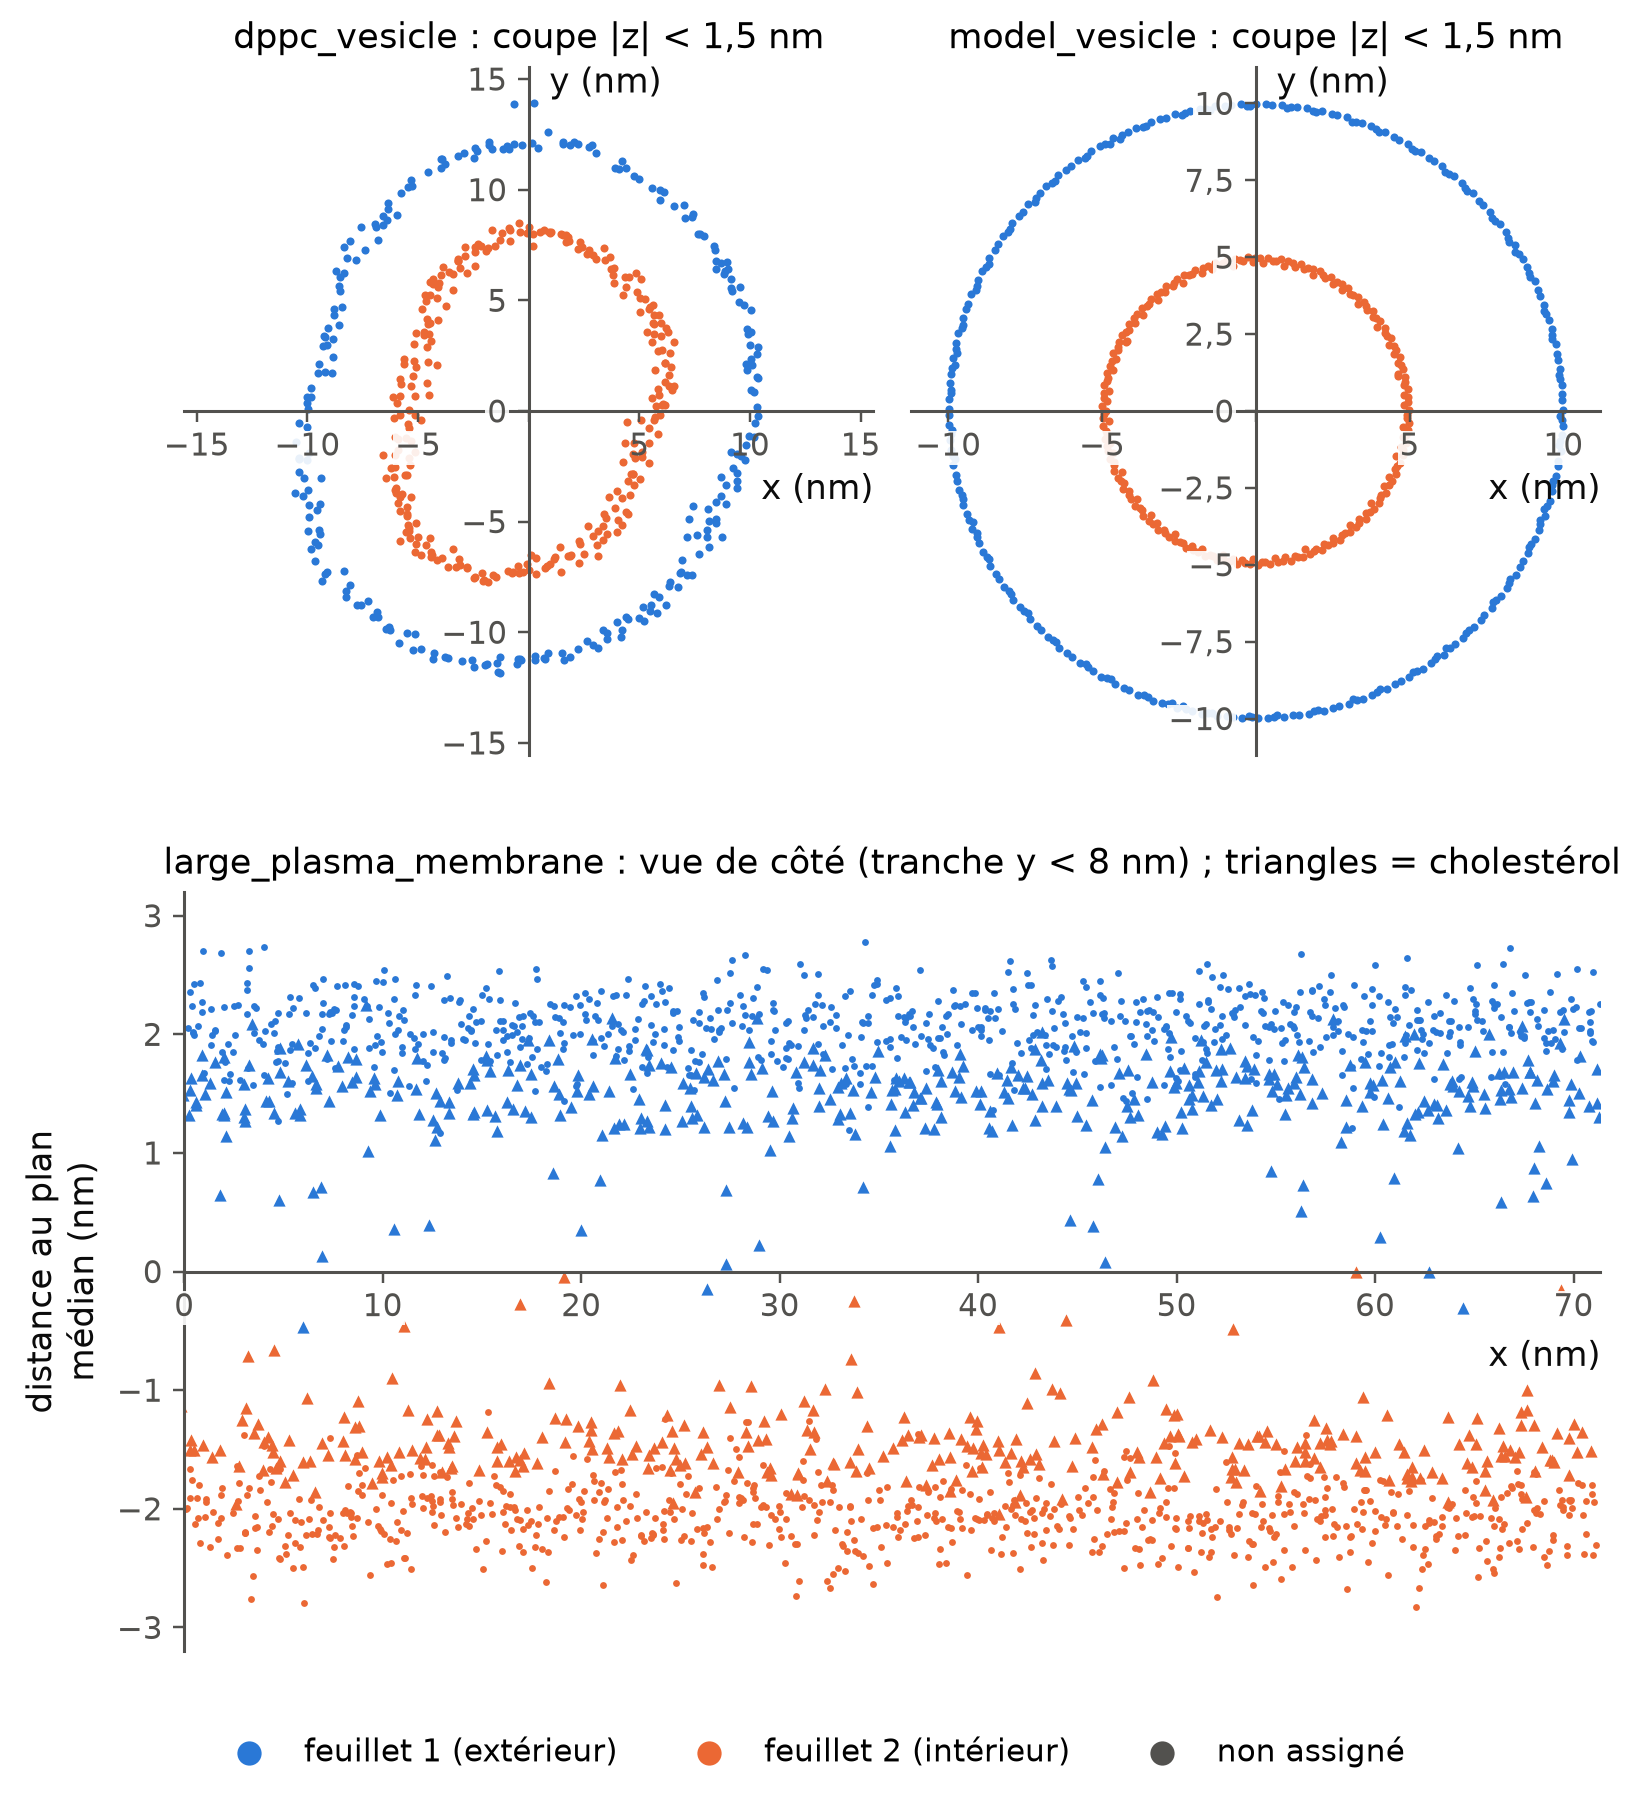
\includegraphics[width=0.92\textwidth]{../../resultats/figures/fig_feuillets.png}
\caption{Feuillets trouvés par la V4 (atomes de référence). À gauche, coupe de la vésicule auto-assemblée
\texttt{dppc\_vesicle} (boîte triclinique, reconstituée à travers les PBC)~; au centre, coupe de la vésicule
modèle~; à droite, vue de côté d'une tranche de la grande membrane plasmique~: les points situés entre les deux
feuillets sont des molécules de cholestérol, assignées selon leur orientation et leur voisinage.}\label{fig:feuillets}
\end{figure}

%=====================================================================
\section{Comparaison sur les structures (point 6)}\label{sec:struct}
%=====================================================================
LeafletFinder a été utilisé avec les mêmes atomes de référence que la V1, avec les PBC activées, d'une part avec son
seuil par défaut (15\,Å) et d'autre part avec le seuil donné par \texttt{optimize\_cutoff}. FATSLiM~0.2.2 a été
utilisé avec ces mêmes atomes comme groupe \texttt{headgroups} et ses paramètres par défaut (seuil de 2\,nm).

\begin{table}[H]\centering\small
\caption{Accord avec la référence (\%). En exposant~: nombre de groupes trouvés par LeafletFinder quand il est
supérieur à 2 (groupes parasites). En gras~: meilleure valeur. LF~=~LeafletFinder~; «~échec~»~:
\texttt{optimize\_cutoff} ne trouve aucun seuil satisfaisant son critère d'équilibre.}\label{tab:accord}
\setlength{\tabcolsep}{4.5pt}
\begin{tabular}{|l|c|c|c|c|c|c|c|c|}\hline
\textbf{Système} & \textbf{V1} & \textbf{V2} & \textbf{V3} & \textbf{V4} & \textbf{V5} & \textbf{LF 15\,Å} & \textbf{LF opt.} & \textbf{FATSLiM}\\\hline
\tabinput{tables/accord.tex}
\end{tabular}
\end{table}

\begin{table}[H]\centering\small
\caption{Nombre de lipides mal assignés (même ordre des colonnes).}\label{tab:erreurs}
\setlength{\tabcolsep}{5pt}
\begin{tabular}{|l|c|c|c|c|c|c|c|c|}\hline
\textbf{Système} & \textbf{V1} & \textbf{V2} & \textbf{V3} & \textbf{V4} & \textbf{V5} & \textbf{LF 15\,Å} & \textbf{LF opt.} & \textbf{FATSLiM}\\\hline
\tabinput{tables/erreurs.tex}
\end{tabular}
\end{table}

\paragraph{Vérification lipide par lipide.} Le script \texttt{scripts/verifier\_resultats.py} relit les feuillets
enregistrés par chaque méthode et les compare, lipide par lipide, aux fichiers \texttt{leaflets.txt}~: il donne pour
chaque méthode le nombre de lipides dans le bon feuillet, dans le mauvais, non assignés ou placés dans un groupe
parasite (\texttt{resultats/verification/resume\_verification.txt}), la liste de chaque lipide mal placé avec sa
position et son orientation (\texttt{<système>\_<méthode>\_erreurs.csv}), un script VMD qui les montre en rouge, et
la figure~\ref{fig:verif}. Il vérifie aussi que les fichiers enregistrés sont identiques à un calcul refait au
moment de la vérification.

\begin{figure}[H]\centering
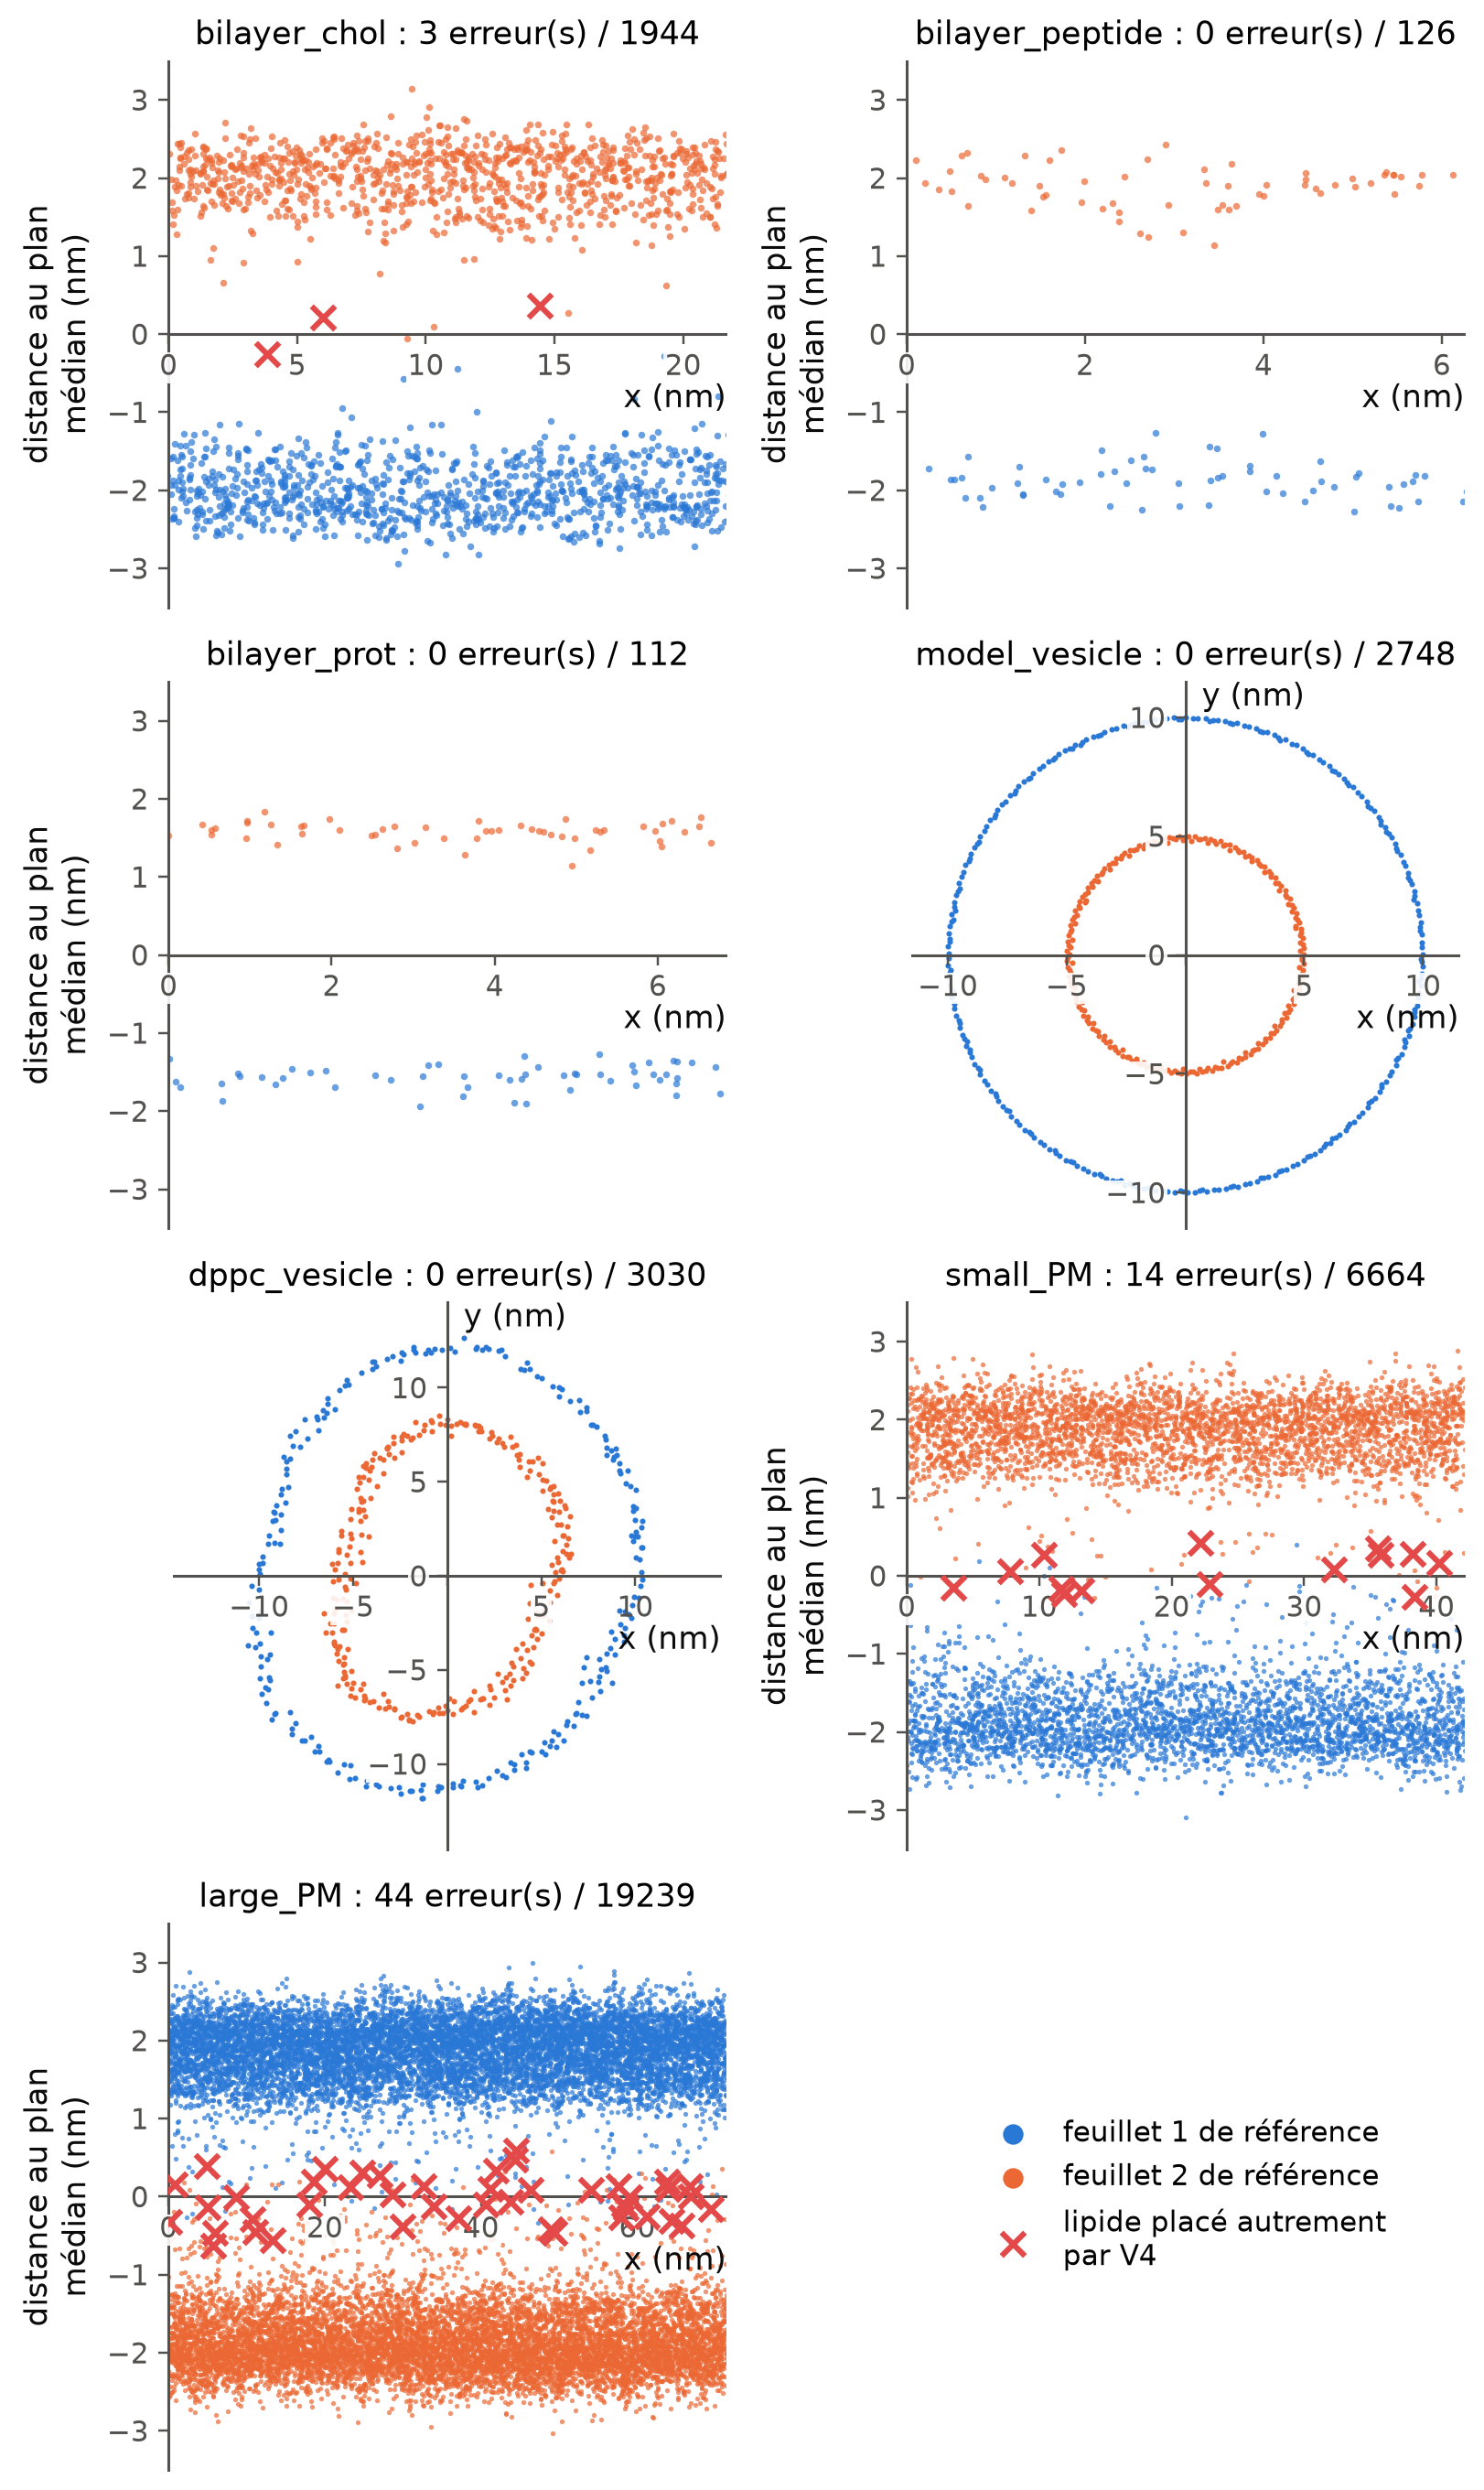
\includegraphics[width=0.70\textwidth]{../../resultats/verification/fig_verification.png}
\caption{Position des lipides mal placés par la V4 (croix rouges) par rapport aux feuillets de référence (bleu,
orange). Membranes planes~: distance de la tête au plan médian local en fonction de $x$~; vésicules~: coupe
équatoriale. Toutes les erreurs sont proches du plan médian.}\label{fig:verif}
\end{figure}

\paragraph{Fiabilité.} Sur les bicouches simples et les vésicules, toutes nos versions sont exactes (100\,\%).
Sur \texttt{bilayer\_chol} et les membranes plasmiques, il reste 2 à 54 désaccords sur 1944 à 19\,239 lipides.
Une analyse détaillée (\texttt{resultats/structures/analyse\_erreurs.txt}) montre qu'\textbf{il s'agit
exclusivement de cholestérols (et de 2 diacylglycérols) dont la tête se trouve à moins de 0,8\,nm du plan médian}
de la bicouche, dont la demi-épaisseur est de 1,8--2\,nm~: ce sont des molécules en cours de \emph{flip-flop}, dont
l'appartenance à un feuillet est intrinsèquement ambiguë. FATSLiM, qui a très probablement servi à produire la
référence, les place «~correctement~» par construction~; sur \texttt{small\_PM}, où il ne coïncide pas
exactement avec la référence, il fait lui-même 12 erreurs contre 14--15 pour nos versions.
LeafletFinder avec son seuil par défaut échoue sur les deux membranes plasmiques~: tous les lipides sont fusionnés
en un seul groupe (51\,\% d'accord). Avec le seuil optimisé, il atteint 98,2--98,5\,\%, mais produit des centaines
de petits groupes parasites (lipides isolés) qu'il n'assigne à aucun feuillet. Il produit aussi 18 groupes sur la
vésicule auto-assemblée (les lipides libres forment des groupes séparés, ce qui est correct). Il n'a pas de mécanisme
de rattachement des lipides isolés ni d'information d'orientation.

\begin{table}[H]\centering\small
\caption{Temps d'analyse d'une structure (ms). Pour V1--V5 et LeafletFinder, minimum sur plusieurs répétitions~;
LF opt. inclut la recherche du seuil par \texttt{optimize\_cutoff}~; FATSLiM~: temps par trame affiché par le
logiciel (résolution 1\,ms).}\label{tab:temps}
\setlength{\tabcolsep}{4pt}
\begin{tabular}{|l|c|c|c|c|c|c|c|c|c|}\hline
& \multicolumn{5}{c|}{\textbf{Nos versions}} & \multicolumn{2}{c|}{\textbf{LeafletFinder}} & \multicolumn{2}{c|}{\textbf{FATSLiM}}\\ \hline
\textbf{Système} & \textbf{V1} & \textbf{V2} & \textbf{V3} & \textbf{V4} & \textbf{V4 12\,thr.} & \textbf{15\,Å} & \textbf{opt.} & \textbf{1\,thr.} & \textbf{12\,thr.}\\\hline
\tabinput{tables/temps.tex}
\end{tabular}
\end{table}

\begin{figure}[H]\centering
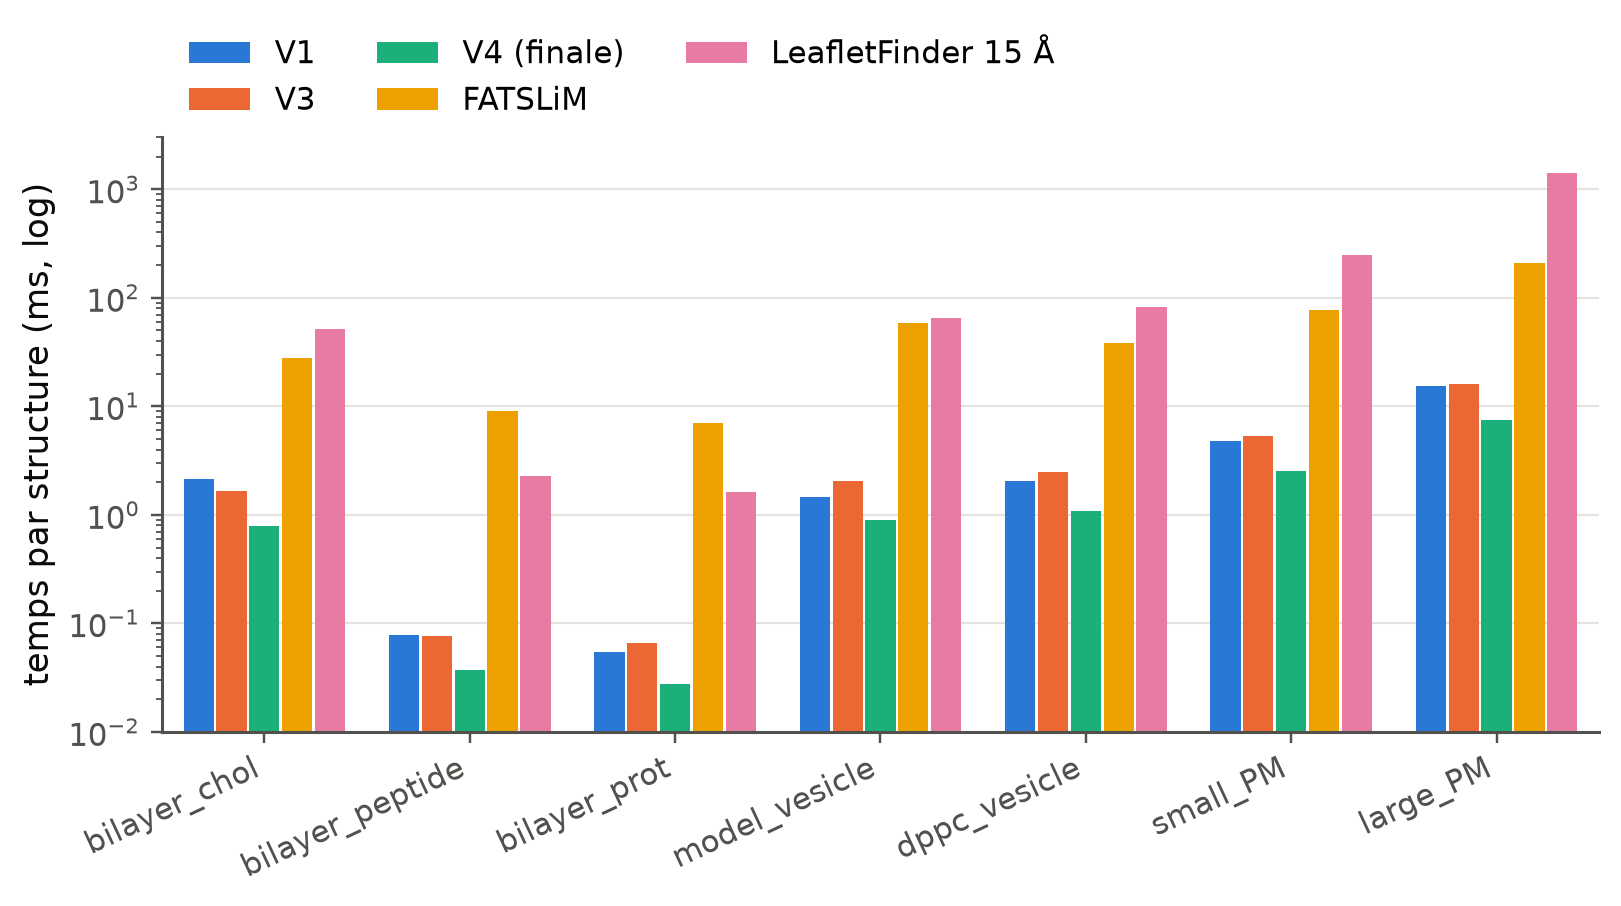
\includegraphics[width=0.95\textwidth]{../../resultats/figures/fig_temps_structures.png}
\caption{Temps d'analyse d'une structure (échelle logarithmique, un thread).}\label{fig:temps}
\end{figure}

\paragraph{Temps de calcul.} La V4 est la plus rapide de nos versions sur toutes les structures de plus de 1000
lipides~; sur les deux petites bicouches (112 et 126 lipides), toutes nos versions prennent moins de 0,1\,ms et les
écarts relèvent du bruit de mesure. Sur la plus grande membrane (19\,239 lipides, 523\,703 particules), la V4 prend
7,5\,ms sur un cœur, soit environ 0,4\,µs par lipide. Elle est 28 à 250 fois plus rapide que FATSLiM sur un thread
(28 fois sur la grande membrane plasmique) et 59 à 185 fois plus rapide que LeafletFinder avec seuil fixe~;
LeafletFinder avec recherche du seuil demande 8 à 42\,s sur les membranes plasmiques, soit un rapport de 3000 à 5500.
Le coût varie linéairement avec le nombre de lipides (figure~\ref{fig:temps}).

\paragraph{Parallélisation.} Sur une seule structure, la parallélisation OpenMP de la recherche de voisins
apporte un gain de 1,45 sur la grande membrane avec 12 threads (figure~\ref{fig:threads}). Il est limité parce que le travail par
trame est très court (quelques ms) et parce que les étapes Union-Find et étiquetage sont séquentielles~; sur les
petits systèmes, le surcoût de création des threads l'emporte. Pour une trajectoire, il est bien plus efficace de
paralléliser \emph{sur les trames} (section~\ref{sec:traj}).

\begin{figure}[H]\centering
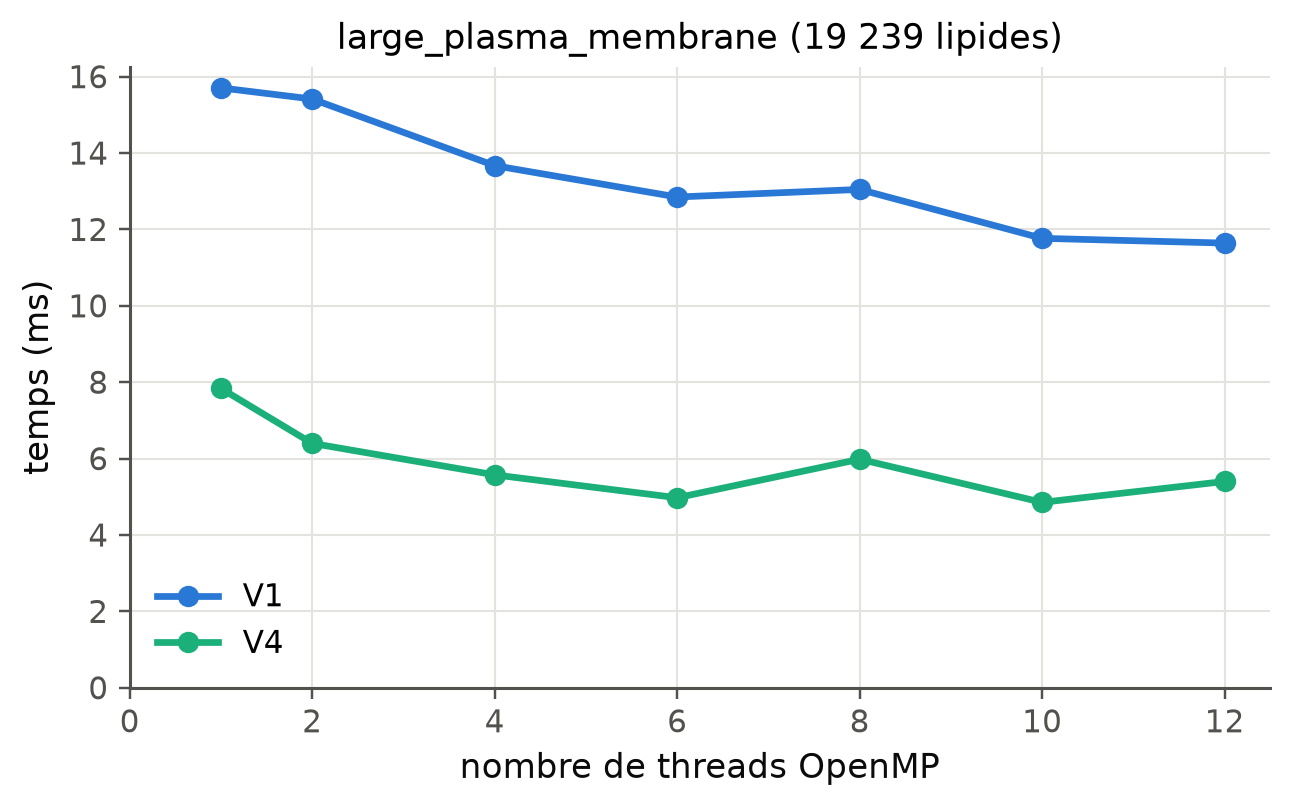
\includegraphics[width=0.62\textwidth]{../../resultats/figures/fig_threads.png}
\caption{Temps d'analyse de la grande membrane plasmique en fonction du nombre de threads OpenMP (processeur
hybride 2 cœurs P + 8 cœurs E).}\label{fig:threads}
\end{figure}

%=====================================================================
\section{Application à la trajectoire (points 5 et 6)}\label{sec:traj}
%=====================================================================
\paragraph{Mise en œuvre.} La trajectoire est lue avec MDAnalysis (formats XTC et TRR) et chaque trame est transmise
au code C++. Le découpage en molécules est lu une fois dans \texttt{prod.tpr}, la surfactine est exclue, et les
atomes de tête sont détectés une seule fois sur la première trame (\TPDetect\,ms~: \texttt{NC3} pour PIPC, le
sucre \texttt{B1} pour GCER, \texttt{ROH} pour le cholestérol). La V4 est ensuite appliquée à chaque trame~; les
numéros de feuillets sont mis en correspondance d'une trame à l'autre et les feuillets de toutes les trames sont
enregistrés (\texttt{resultats/trajectoire\_surfactine\_*/feuillets\_V4.txt}). L'exécutable C++ peut aussi traiter
seul une trajectoire au format GRO multi-trames (lecture comprise), en répartissant les trames entre les threads
(option \texttt{-P}).

\paragraph{Comment juger la fiabilité sans référence~?} La trajectoire n'est pas accompagnée de fichier
\texttt{leaflets.txt}. Nous utilisons trois contrôles indépendants~:
\begin{enumerate}
\item l'accord avec FATSLiM et avec la V1, méthodes fondées sur d'autres principes (normales par ACP, seuil
automatique)~;
\item une \emph{référence géométrique}~: la membrane étant plane, un lipide appartient au feuillet supérieur si sa
tête est au-dessus du plan médian \emph{local} (milieu entre la couche de têtes du haut et celle du bas, estimé sur
une grille d'environ 3\,nm$\times$3\,nm, ce qui suit les ondulations)~; validée sur les cinq structures planes, cette
référence concorde à 99,6--100\,\% avec les fichiers \texttt{leaflets.txt}~; elle est ambiguë pour les molécules
proches du plan médian~;
\item la cohérence temporelle~: en 20\,µs, les phospholipides et les glycolipides ne doivent pratiquement jamais
changer de feuillet (\emph{flip-flop} de l'ordre de l'heure), alors que le cholestérol bascule rapidement.
\end{enumerate}

\begin{table}[H]\centering\small
\caption{Temps d'analyse des trajectoires (un thread sauf mention). V4 total~: temps cumulé sur toutes les trames~;
dernière colonne~: temps estimé pour 100\,000 trames avec la V4, les trames étant réparties sur \TNcpu~threads (lecture
du fichier exclue).}\label{tab:trajtemps}
\setlength{\tabcolsep}{4pt}
\begin{tabular}{|l|r|r|r|r|r|r|r|}\hline
& \textbf{V4 total} & \multicolumn{4}{c|}{\textbf{ms par trame}} & \textbf{V4 //} & \textbf{100\,000}\\ \cline{3-6}
\textbf{Trajectoire} & \textbf{(ms)} & \textbf{V4} & \textbf{V1} & \textbf{LF 15\,Å} & \textbf{FATSLiM} & \textbf{ms/trame} & \textbf{trames (s)}\\\hline
\tabinput{tables/traj_temps.tex}
\end{tabular}
\end{table}

\begin{table}[H]\centering\small
\caption{Fiabilité sur les trajectoires (moyenne sur les trames, \%). Gauche~: accord de la V4 avec les autres
méthodes. Droite~: accord de chaque méthode avec la référence géométrique (plan médian local).}\label{tab:trajacc}
\setlength{\tabcolsep}{4pt}
\begin{tabular}{|l|c|c|c|c|c|c|c|}\hline
& \multicolumn{3}{c|}{\textbf{V4 comparée à}} & \multicolumn{4}{c|}{\textbf{Référence géométrique}}\\ \hline
\textbf{Trajectoire} & \textbf{FATSLiM} & \textbf{V1} & \textbf{LF} & \textbf{V4} & \textbf{V1} & \textbf{FATSLiM} & \textbf{LF}\\\hline
\tabinput{tables/traj_accord.tex}
\end{tabular}
\end{table}

\paragraph{Temps de calcul (point 5).} Sur les \TPTrames~trames de \texttt{prod1.xtc}, la V4 analyse une trame de
\TPLipides~lipides en \TPVq\,ms, soit \TPVtot\,s pour toute la trajectoire sur un cœur, contre \TPFat\,s pour
FATSLiM et \TPLF\,s pour LeafletFinder (tableau~\ref{tab:trajtemps}, figure~\ref{fig:trajtemps}). Le temps par trame
est stable d'une trame à l'autre. En répartissant les trames sur les \TNcpu~threads, le débit passe de \TPSeqHz~à
\TPParHz~trames/s~: une trajectoire de 100\,000 trames de ce système serait analysée en environ \TPExtPar\,s (\TPExtSeq\,s
sur un cœur), hors lecture du fichier (\TPLecture\,ms par trame pour décompresser le XTC avec MDAnalysis, soit
davantage que l'analyse elle-même). La durée « de l'ordre de la seconde » par trame citée dans l'énoncé conduirait
à environ 28~heures.

\begin{figure}[H]\centering
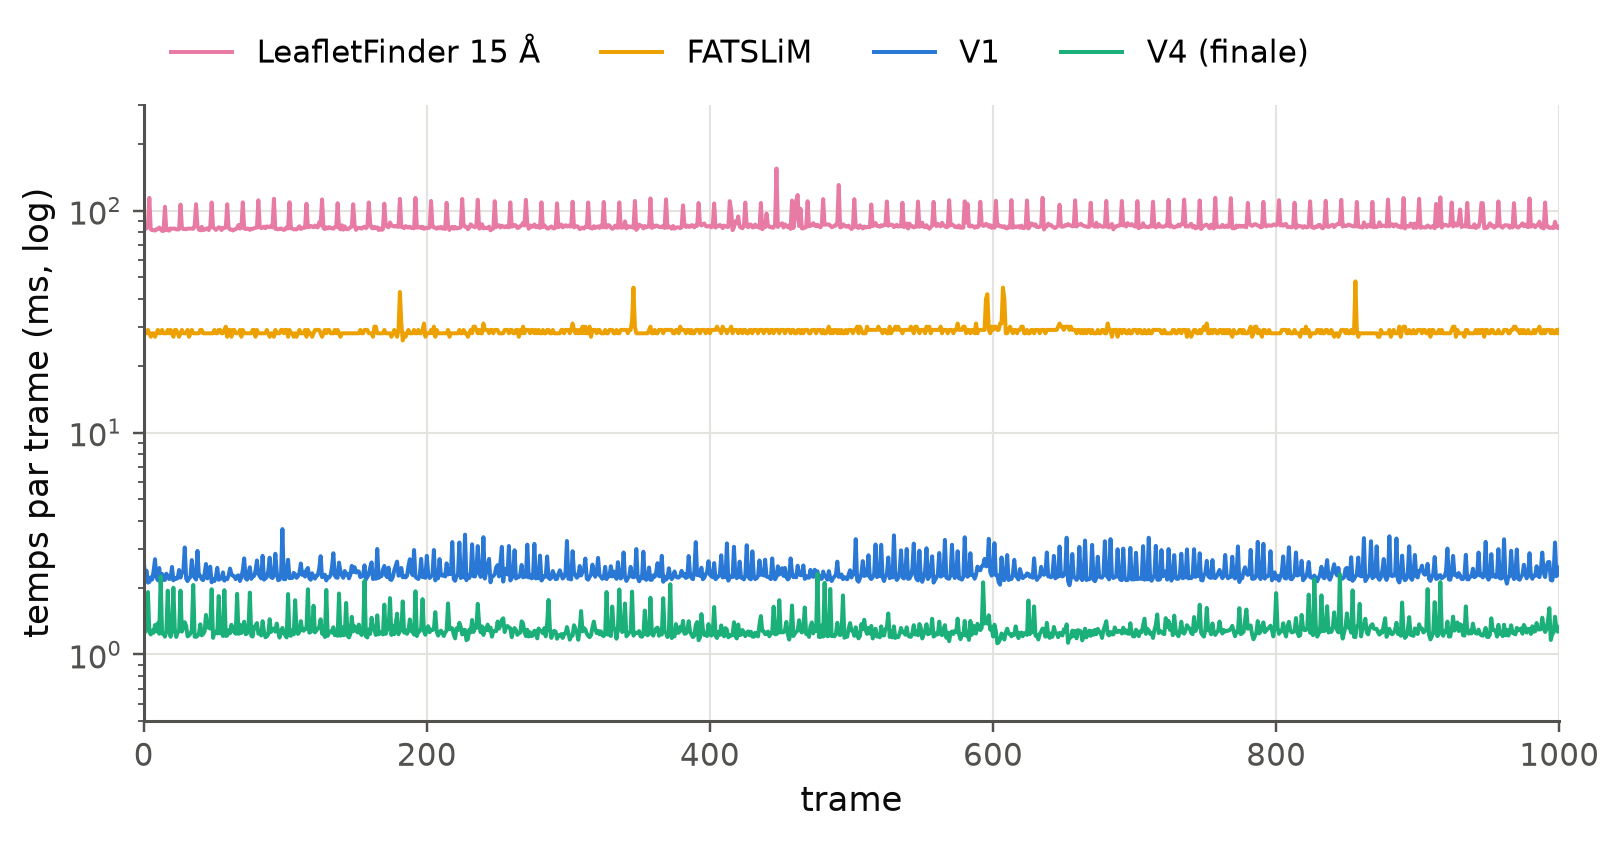
\includegraphics[width=0.92\textwidth]{../../resultats/figures/fig_trajectoire_temps.png}
\caption{Temps d'analyse par trame le long de \texttt{prod1.xtc} (1001 trames, échelle logarithmique).}\label{fig:trajtemps}
\end{figure}

\paragraph{Fiabilité (point 6).} Sur les trois trajectoires de la surfactine, la V4 attribue le même feuillet que
FATSLiM à \TPAccFat\,\% des lipides en moyenne (au moins \TPAccFatMin\,\% sur chaque trame) et le même que la V1 à
99,8\,\%. Face à la référence géométrique, V4, V1 et FATSLiM obtiennent tous 99,6 à 99,7\,\%
(tableau~\ref{tab:trajacc}). Les désaccords avec cette référence sont uniquement des cholestérols, environ 10 par
trame sur 3040 lipides, dont la tête est à 0,17\,nm en médiane du plan médian local (au plus 1,1\,nm), là où
« au-dessus » et « au-dessous » n'ont plus de sens (\texttt{resultats/trajectoire\_surfactine\_20us/analyse\_types.txt}).
Aucun PIPC ni GCER n'est en désaccord.
LeafletFinder, avec son seuil par défaut, fusionne les deux feuillets sur 96\,\% des trames (1043 sur 1083~; environ
52\,\% d'accord en moyenne), comme sur les membranes plasmiques~: il ne sépare correctement les feuillets que sur
les rares trames où aucun lipide ne fait le pont entre eux. Aucune trame n'est fusionnée par la V4 (\TPFusions~trame sur \TPTrames).

\paragraph{Ce que montre la trajectoire.} Sur la production de 20\,µs (figure~\ref{fig:surf20}), les deux feuillets
gardent environ 1520 lipides chacun. Entre deux trames séparées de 1\,µs, en moyenne \TLChgMoy~lipides changent de
feuillet~: \textbf{ce sont tous des cholestérols} (environ la moitié des 608 cholestérols), alors qu'aucun PIPC ni
aucun GCER ne change de feuillet en 20\,µs. C'est le comportement attendu (basculement rapide du cholestérol en
Martini, phospholipides stables) et c'est un argument fort en faveur de la fiabilité de l'assignation. Sur
\texttt{prod1.xtc}, dont les trames sont espacées de 5\,ps, environ \TPChgMoy~cholestérols changent d'assignation
d'une trame à l'autre (0,8\,\% des cholestérols)~; un vrai basculement étant impossible en 5\,ps, il s'agit de
l'ambiguïté résiduelle sur ces molécules. Toutes les méthodes la présentent~: 4,3 cholestérols par trame pour la V1,
4,7 pour la V3, 4,8 pour la V4 et 7,0 pour FATSLiM, qui fait aussi changer d'assignation quelques PIPC et GCER, ce
que la V4 ne fait jamais (\texttt{resultats/trajectoire\_surfactine\_prod1/clignotement.txt}).

\begin{figure}[H]\centering
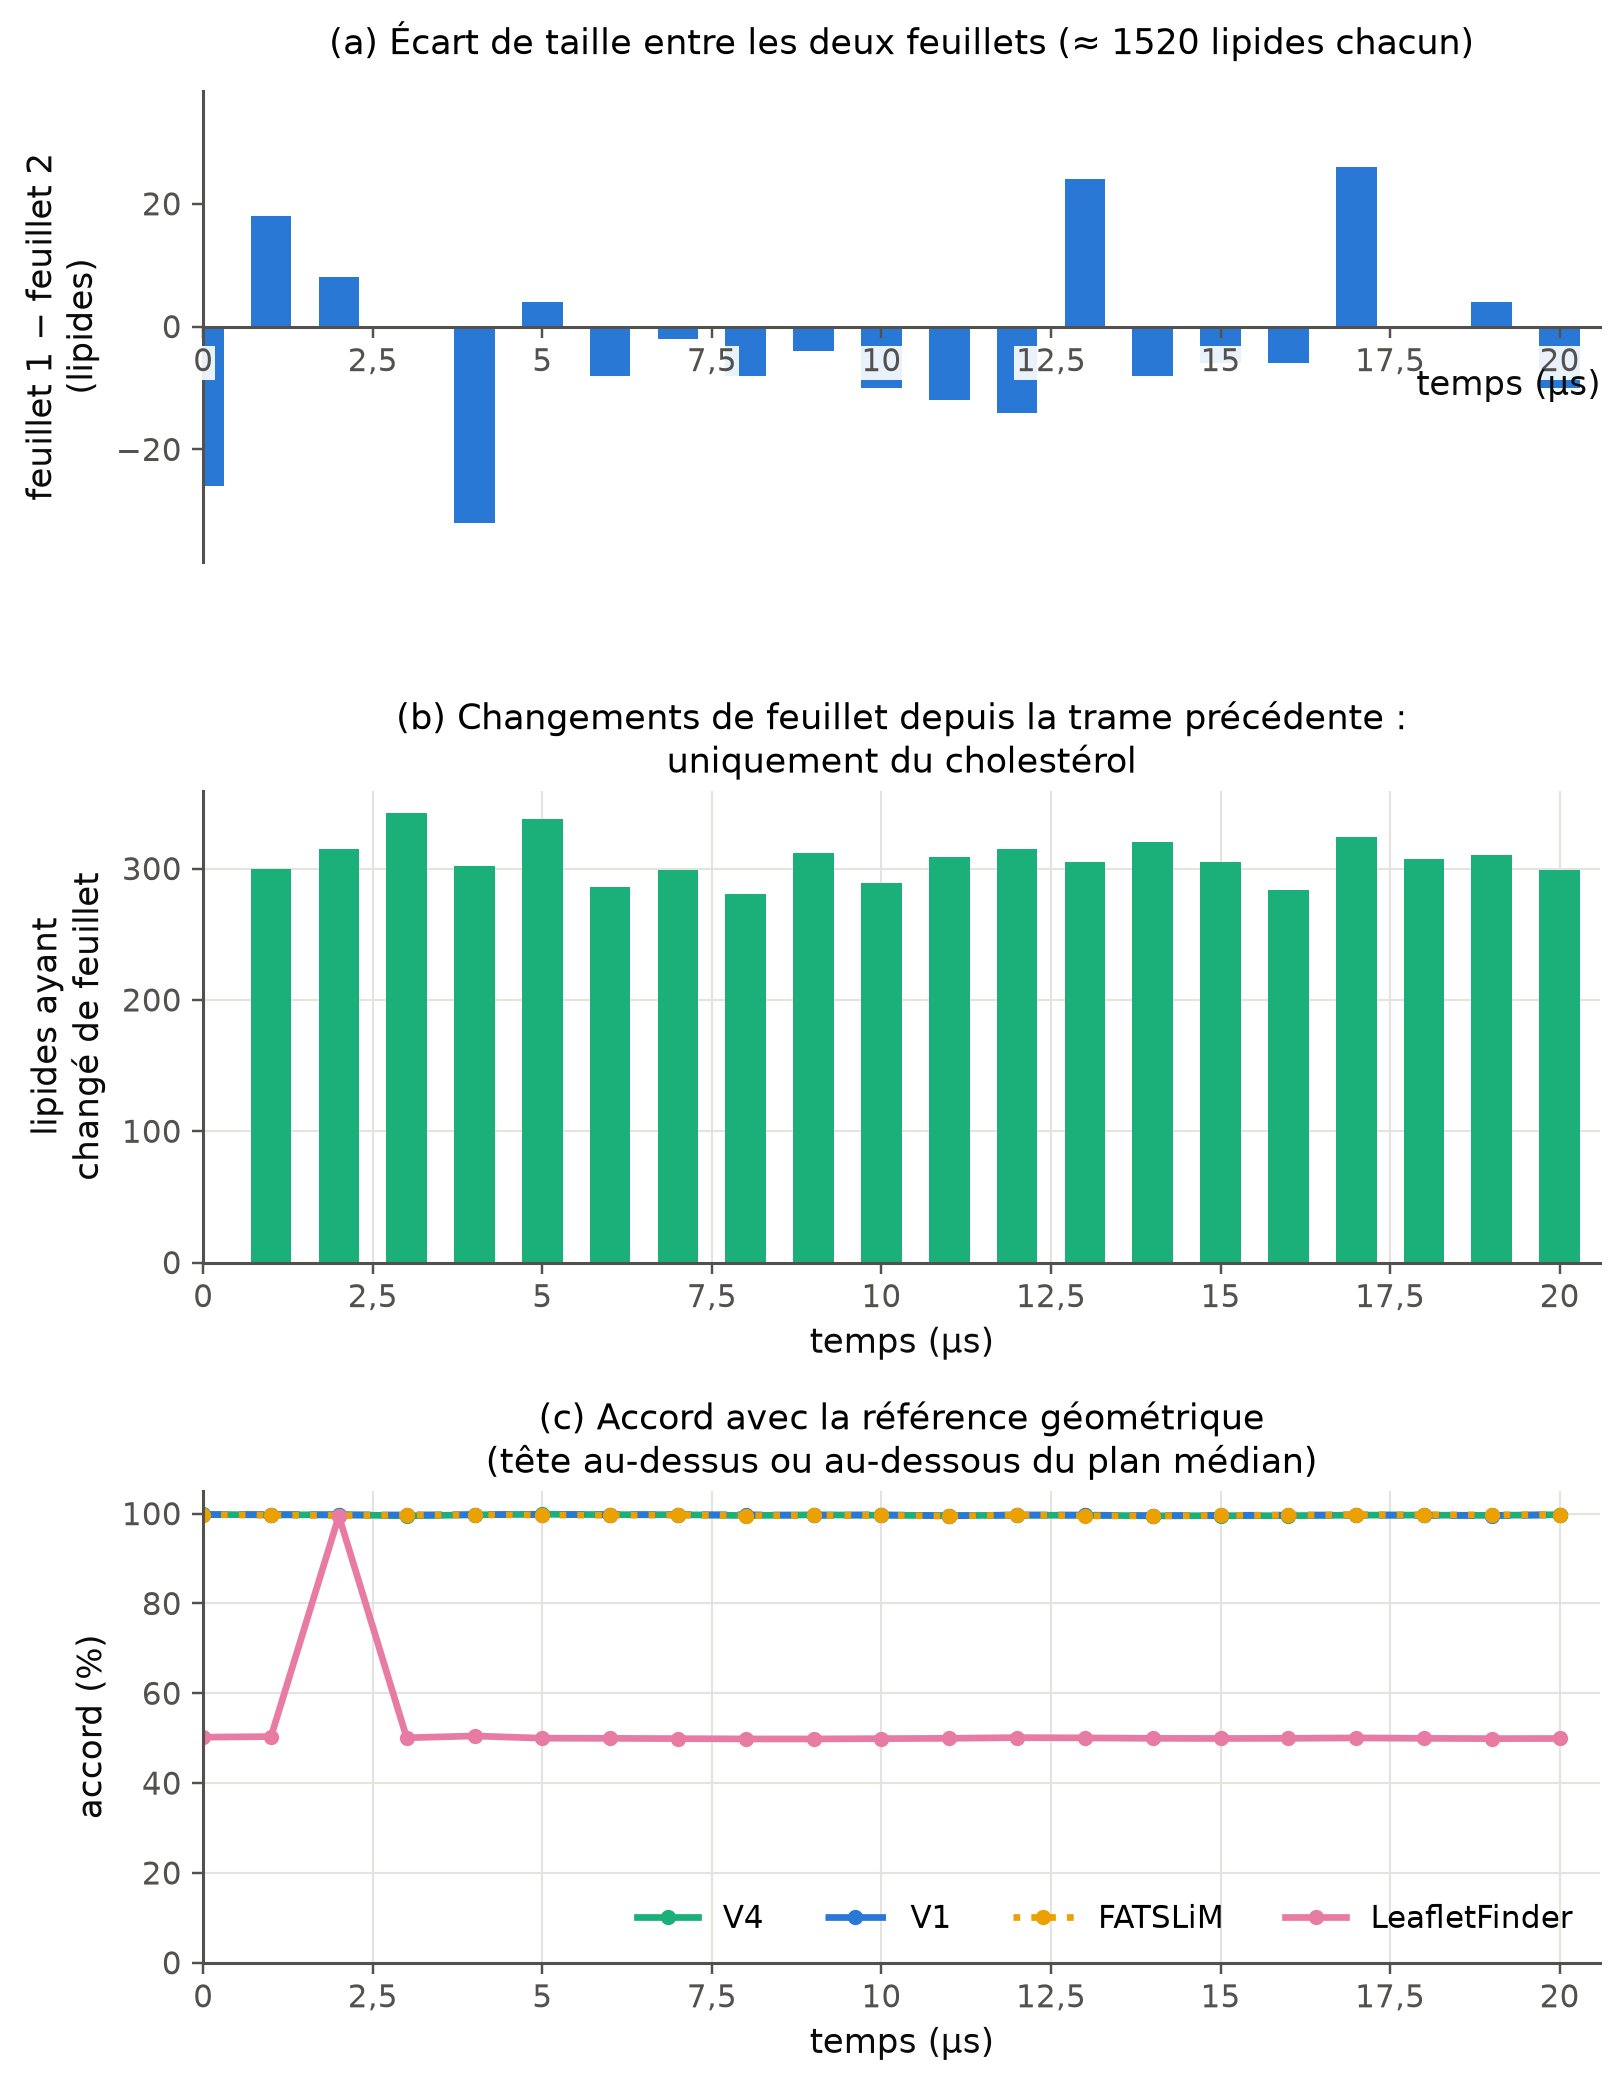
\includegraphics[width=0.85\textwidth]{../../resultats/figures/fig_surfactine_20us.png}
\caption{Production de 20\,µs (1 trame/µs). Gauche~: taille des deux feuillets. Centre~: nombre de lipides ayant
changé de feuillet depuis la trame précédente (uniquement des cholestérols). Droite~: accord avec la référence
géométrique.}\label{fig:surf20}
\end{figure}

\begin{figure}[H]\centering
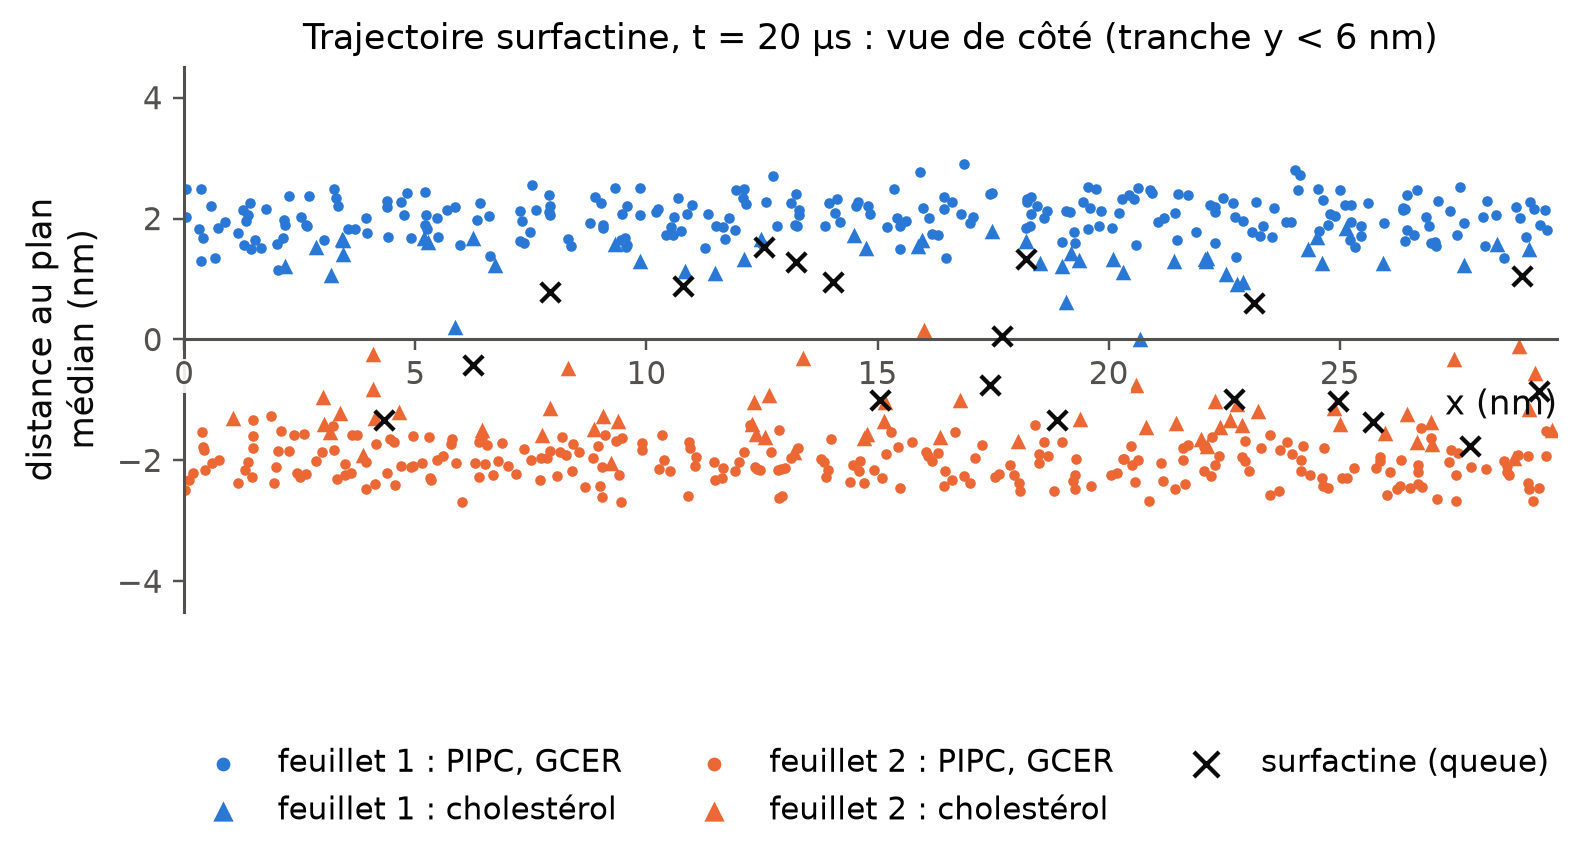
\includegraphics[width=0.95\textwidth]{../../resultats/figures/fig_surfactine_vue.png}
\caption{Feuillets trouvés par la V4 sur la dernière trame (20\,µs), vue de côté d'une tranche de la membrane~:
têtes des phospholipides et glycolipides (points), cholestérols (triangles) et queues de surfactine (croix).}\label{fig:surfvue}
\end{figure}

\paragraph{Validation sur une autre trajectoire.} Avant de disposer de la trajectoire du cours, la chaîne a été mise
au point sur une trajectoire de la vésicule DPPC (11 trames, données de test de FATSLiM)~: accord de
\TDAccRef\,\% avec la référence à la trame~0 et de \TDAccFat\,\% avec FATSLiM, pour \TDVq\,ms par trame
(tableaux~\ref{tab:trajtemps} et~\ref{tab:trajacc}, dernière ligne).


%=====================================================================
\section{Discussion et limites}
%=====================================================================
\begin{itemize}
\item \textbf{Lipides ambigus.} Les seules erreurs restantes concernent des molécules au plan médian. Pour une
analyse ultérieure (aire par lipide, épaisseur), il peut être préférable de les déclarer «~non assignées~»~: la
cohérence $q_i$ calculée par la V4 fournit naturellement cet indicateur.
\item \textbf{Paramètres.} La V4 utilise des seuils fixes (1,5\,nm, $\cos\theta=0{,}5$, $q\geq0{,}5$) valables pour
les représentations CG et UA testées. Pour des systèmes tout-atome, on pourrait les exprimer en multiples de la
distance moyenne entre têtes voisines, mesurée automatiquement.
\item \textbf{Systèmes multiples.} Le programme sépare naturellement plusieurs membranes (composantes distinctes)~;
nous ne l'avons pas évalué sur des empilements de bicouches, absents des données fournies.
\item \textbf{Cohérence temporelle.} L'analyse est faite trame par trame, sans mémoire~: quelques cholestérols
ambigus changent d'assignation d'une trame à l'autre (section~\ref{sec:traj}). Un lissage temporel (ne valider un
changement de feuillet que s'il persiste sur quelques trames) éliminerait ce bruit sans coût notable.
\item \textbf{Topologie.} Pour des lipides écrits sur plusieurs résidus (Martini~3), le découpage en molécules doit
venir du fichier \texttt{.tpr}~; sans lui, un glucosylcéramide serait compté comme deux molécules.
\item \textbf{Données de la trajectoire.} Le fichier \texttt{prod.trr} est tronqué (61 trames lisibles) et la
production complète n'est disponible qu'à raison d'une trame par microseconde (\texttt{prod\_dt1000ns.xtc})~; la
mesure de temps la plus représentative est donc celle de \texttt{prod1.xtc} (1001 trames).
\item \textbf{Conditions de mesure.} Les temps finaux ont été mesurés sur batterie~; le script
\texttt{resultats/relance\_tout.sh} permet de les refaire dans de meilleures conditions.
\item \textbf{Référence.} La référence semble produite par FATSLiM~: un accord de 100\,\% avec elle n'est pas une
vérité absolue pour les molécules en cours de \emph{flip-flop}.
\end{itemize}

%=====================================================================
\section*{Conclusion}
\addcontentsline{toc}{section}{Conclusion}
%=====================================================================
Nous avons réalisé les quatre versions demandées. La recherche automatique du seuil (V1) rend l'approche par
graphe fiable, mais révèle sa fragilité sur les membranes complexes (plateau de 0,25\,nm). La détection
automatique de l'atome de tête par un critère d'exposition (V2) supprime toute connaissance préalable de la chimie
des lipides. L'orientation et la normale locale (V3) suppriment la sensibilité au seuil. La version finale (V4) ne
garde que l'essentiel~: atome de tête détecté, orientation lissée sur un voisinage de 1,5\,nm, graphe des lipides
cohérents et rattachement des lipides ambigus. Elle atteint 99,77--100\,\% d'accord, équivalent à FATSLiM, en
0,4\,µs par lipide, soit un à deux ordres de grandeur plus vite que FATSLiM et LeafletFinder. Elle permet
d'analyser une trajectoire de 100\,000 trames en quelques dizaines de secondes.

\addcontentsline{toc}{section}{Références}
\begin{thebibliography}{9}
\bibitem{mda} N.~Michaud-Agrawal, E.~J.~Denning, T.~B.~Woolf, O.~Beckstein, \emph{MDAnalysis: A toolkit for the
analysis of molecular dynamics simulations}, J.~Comput.~Chem. 32(10), 2319--2327 (2011).
\bibitem{fatslim} S.~Buchoux, \emph{FATSLiM: a fast and robust software to analyze MD simulations of membranes},
Bioinformatics 33(1), 133--134 (2017).
\bibitem{limonada} LIMONADA, base de données de lipides et de membranes, \url{https://limonada.univ-reims.fr}.
\end{thebibliography}

%=====================================================================
\section*{Fichiers joints et utilisation}\label{sec:usage}
\addcontentsline{toc}{section}{Fichiers joints et utilisation}
%=====================================================================
\begin{lstlisting}
src/leaflet.cpp               code C++ (versions 1 à 5, exécutable + bibliothèque)
Makefile                      compilation (make)
scripts/lfpy.py               interface Python (ctypes) + évaluation
scripts/benchmark_structures.py  points 1-4 et 6 sur les 7 structures
scripts/run_trajectory.py     points 5 et 6 sur une trajectoire
scripts/xtc_to_gro.py         conversion XTC -> GRO multi-trames (pour bin/leaflet)
scripts/tpr_molsizes.py       découpage en molécules depuis un TPR (pour bin/leaflet)
scripts/analyse_types_trajectoire.py  changements de feuillet par type de lipide
Surfactine-R1/                trajectoire du cours (GROMACS, Martini 3)
scripts/make_figures.py, make_tables.py   figures et tableaux du rapport
resultats/structures/         CSV, feuillets trouvés par chaque méthode
resultats/trajectoire*/       résultats par trame, résumés (DPPC + surfactine)
resultats/figures/            figures
doc_Projet/rapport/           ce rapport (rapport.tex, rapport.pdf)
\end{lstlisting}

\paragraph{Compilation et exécution d'une structure.}
\begin{lstlisting}
make
./bin/leaflet -f Projet3/bilayer_chol/bilayer_chol.gro -m 4 -o feuillets.txt \
              -r Projet3/bilayer_chol/leaflets.txt
# -m 1..5 : version ; -c seuil (nm) ; -t threads ; --heads : atomes de tête détectés
\end{lstlisting}

\paragraph{Trajectoire du cours (surfactine).}
\begin{lstlisting}
.venv/bin/python scripts/run_trajectory.py --gro Surfactine-R1/prod.gro \
    --traj Surfactine-R1/prod1.xtc --tpr Surfactine-R1/prod.tpr --exclude S14 --zref \
    --out trajectoire_surfactine_prod1
# exécutable seul : découpage en molécules issu du TPR, surfactine exclue
.venv/bin/python scripts/tpr_molsizes.py Surfactine-R1/prod.tpr molsizes.txt
./bin/leaflet -f Surfactine-R1/prod.gro --molsizes molsizes.txt -x S14
\end{lstlisting}

\paragraph{Autre trajectoire.}
\begin{lstlisting}
.venv/bin/python scripts/run_trajectory.py --gro structure.gro --traj trajectoire.xtc
# ou, avec l'exécutable seul (lecture comprise, trames en parallèle) :
.venv/bin/python scripts/xtc_to_gro.py structure.gro trajectoire.xtc traj.gro
./bin/leaflet -f traj.gro -P -t 12 -s par_trame.csv
\end{lstlisting}

\paragraph{Reproduction de l'ensemble des résultats et du rapport.}
\begin{lstlisting}
.venv/bin/python scripts/benchmark_structures.py
.venv/bin/python scripts/run_trajectory.py
.venv/bin/python scripts/make_figures.py && .venv/bin/python scripts/make_tables.py
resultats/relance_tout.sh        # toutes les mesures (structures + trajectoires)
cd doc_Projet/rapport && pdflatex rapport.tex && pdflatex rapport.tex
\end{lstlisting}

\end{document}
